
% License:
% CC BY-NC-SA 3.0 (http://creativecommons.org/licenses/by-nc-sa/3.0/)
%
%%%%%%%%%%%%%%%%%%%%%%%%%%%%%%%%%%%%%%%%%

%----------------------------------------------------------------------------------------
%	PACKAGES AND OTHER DOCUMENT CONFIGURATIONS
%----------------------------------------------------------------------------------------

\documentclass[paper=a4, fontsize=11pt]{scrartcl} % A4 paper and 11pt font size

\usepackage[T1]{fontenc} % Use 8-bit encoding that has 256 glyphs
\usepackage{fourier} % Use the Adobe Utopia font for the document
\usepackage[UKenglish]{babel} % English language/hyphenation
\usepackage{amsmath,amsfonts,amsthm} % Math packages
\usepackage{physics}
\usepackage{caption}
\usepackage{subcaption}
\usepackage{graphicx}
\usepackage{bm}
\usepackage{listings}
\usepackage{gensymb}
\usepackage{color}
\usepackage{wrapfig}
\usepackage[normalem]{ulem}
\usepackage{float}
\usepackage{blindtext} %for enumerations
\usepackage[]{hyperref}  %link colour
\usepackage{sectsty} % Allows customizing section commands
\allsectionsfont{\centering \normalfont\scshape} % Make all sections centered, the default font and small caps

\usepackage{fancyhdr} % Custom headers and footers
\pagestyle{fancyplain} % Makes all pages in the document conform to the custom headers and footers
\fancyhead{} % No page header - if you want one, create it in the same way as the footers below
\fancyfoot[L]{} % Empty left footer
\fancyfoot[C]{} % Empty center footer
\fancyfoot[C]{\thepage} % Page numbering for right footer
\renewcommand{\headrulewidth}{0pt} % Remove header underlines
\renewcommand{\footrulewidth}{0pt} % Remove footer underlines
\newcommand{\latex}{\LaTeX\xspace} % Neater LaTeX symbol
\setlength{\headheight}{13.6pt} % Customize the height of the header

\numberwithin{equation}{section} % Number equations within sections (i.e. 1.1, 1.2, 2.1, 2.2 instead of 1, 2, 3, 4)
\numberwithin{figure}{section} % Number figures within sections (i.e. 1.1, 1.2, 2.1, 2.2 instead of 1, 2, 3, 4)
\numberwithin{table}{section} % Number tables within sections (i.e. 1.1, 1.2, 2.1, 2.2 instead of 1, 2, 3, 4)

\setlength\parskip{4pt}

%----------------------------------------------------------------------------------------
%	TITLE SECTION
%----------------------------------------------------------------------------------------

\newcommand{\horrule}[1]{\rule{\linewidth}{#1}} % Create horizontal rule command with 1 argument of height

\title{	
\normalfont \normalsize 
\Large{\textsc{Lancaster University}} \\ [20pt]
\normalsize{\textsc{Phys379 Group Project}} \\ [15pt]
\horrule{0.5pt} \\[0.4cm] % Thin top horizontal rule
\huge  Wildfire Simulation using Cellular Automata: \\ Case  Study of Marysville, Australia
\horrule{2pt} \\[0.5cm] % Thick bottom horizontal rule
}

\author{J. Majaniemi, J. Thomas, A. Baxter and A. Berry}

\date{\normalsize\today}

\begin{document}
\maketitle

\begin{abstract}

{\indent{\Large Abstract} }\\
 
We stage a novel cellular automata model describing wildfire dynamics under the environmental factors of wind speed and direction, surface elevation and spotting. Underlying mechanisms of wildfires are scrutinized and strong relations are constructed to describe the rate and manner in which wildfires spread across heterogeneous landscapes. Further, we perform a case study of the 2009 Black Saturday bushfires in Murrindindi, Australia, by simulating these events using our cellular automata model. Results yielded are compared to historical data from these fires, consequently demonstrating the potential applications in fire modelling and risk-management.

\end{abstract}

\newpage
\tableofcontents

%----------Contents--------------------------

\newpage
\section{Introduction} \label{introduction}

Wildfires are dramatic, destructive and evolve in an almost chaotic manner. They form part of the natural ecological system of our planet, but with advancing global temperatures and imbalances occurring in local environments, they may become more common place in everyday life for high risk regions \cite{JTAba_APWil}. Hence a fundamental understanding of their genesis and characteristics may be essential in limiting the damage caused. It is here we will investigate what the influential characteristics of wildfires are without taking the traditional scientific route of direct physical experiment. We will instead be taking the theoretical approach of simulation.\newline \indent The framework for our simulation is cellular automata, which has been widely studied and successfully applied in past research on living and dynamic systems \cite{CA_1,CA_2}. Cellular automata has been used to model wildfires numerous times before \cite{Aleksandridis_2008,CA-fire_2}, and we will test a novel variation of this modelling system to investigate if it can produce a wildfire simulation of specific parameters. In particular, we explore whether it can offer results akin to historical wildfire data when applied to past geographical source data.\newline \indent To obtain an understanding of the nature of the parameters we are trying to replicate, we can imagine starting a small fire at the corner of this paper. We can now probe into the way in which the fire spreads depending on a collection of factors: the type and thickness of the paper, folds and undulations in the paper, airflow across the surface of the paper and embers resulting from previously burnt regions. All of these have legitimate observable effects on the pattern and rate of burn, and combinations of them begin to give a sense of complexity which was probably not first perceived when introducing the simple concept of burning paper. \newline \indent Developing our image to a geographical scale now leads us to consider parameters such as flammability, topography and wind. We wish to know how accurately these parameters can be modelled via simulation and whether any relations can be derived that explain the attributes. Once a foundation of the principles of cellular automata and wildfire modelling are set in Sections \ref{CA_Principles} and \ref{Modelling_Wildfire} respectively, we develop the methodology behind our model in Section \ref{methodology}. We investigate the proportional influence of different parameters on the effect of wildfire spread, later finding that elevation can decrease the probability of ignition by a factor of 10 in our model with specific environments. Yet the strength and direction of wind highly coerces the behaviour of fire spread, either completely stunting the fires ability to spread or being a determining factor in where the fire spreads.\newline \indent After determining the results that the basis of our model offers in Section \ref{results_1}, we then apply it to real geographical and vegetation data from the Murrindindi Shire in Australia in Section \ref{results_2}. We quantify how accurately our model can replicate the 2009 "Black Saturday Bushfires" under the influence of various environmental parameters, and compare the results of our simulation to historical data. Ultimately it is found that wind again plays a primary role in the core behaviour of the wildfire and provides the largest step in driving the model to more accurately represent the actual events. Wind also becomes a key limiting factor in our model, as its dynamic nature is approximately fixed to a single speed and direction for the duration of the simulation, in turn restricting the true course of the wildfire.

\newpage
\section{Background}\label{background}
\subsection{Principles of Cellular Automata}\label{CA_Principles}

A cellular automaton (CA) is a discrete model of cells arranged in a grid that possesses a set of given states. The state of each cell evolves over a series of time steps according to a set of rules that depend on the states of neighbouring cells. These rules can be applied as many times as required, simulating the evolution of a system over time. \newline \indent In the 1980s, Stephen Wolfram conducted comprehensive studies into elementary cellular automata. An elementary CA works based on two possible states, represented by either a 0 or a 1. Wolfram found that there are 256 different possible rules for elementary CA, each of which is indexed by a unique binary number \cite{wolfram1986theory}. Despite the simplicity of the model, rule number 30 exhibits chaotic behaviour, and can be used as a random number generator \cite{Wolfram_2002}. In Figure \ref{rule190} we observe the elementary cellular automaton for Wolfram's rule 190.

\begin{figure}[h!]
\centering
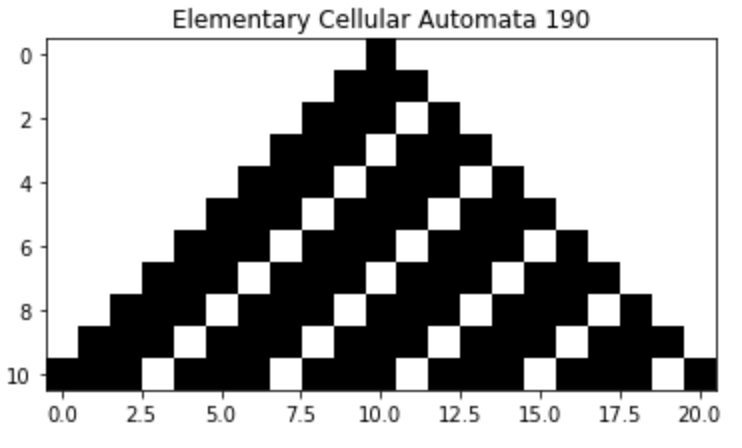
\includegraphics[width=0.5\textwidth]{Figures/cell.png}\caption{An example of an elementary CA using Wolfram's rule 190 for 10 time steps \cite{wolfram1986theory}. White squares represent 0 and black squares represent 1. Each horizontal line represents a different time step, with the initial time step having a '1' binary state at position 10.0 on the x-axis.}\label{rule190}
\end{figure} 

\noindent Cellular automata can be defined in arbitrarily many dimensions. A two-dimensional CA is composed of a rectangular grid of cells; the state of each cell is updated in discrete time steps depending on a particular rule set. The collection of cells surrounding any particular cell is known as the neighbourhood, and the values of the neighbourhood determine the future state of a cell. Two commonly used  neighbourhoods in 2D cellular automata are the \textit{von Neumann neighbourhood} \cite{wolfram1986theory} and the \textit{Moore neighbourhood} \cite{101917}, illustrated in Figure \ref{hoods}. The former is composed of a central cell and the 4 cells adjacent to it, while the latter is composed of a central cell and the 8 cells surrounding it.\newline \indent The advantage of a small neighbourhood is computation speed: there are $50\%$ fewer values required to look up in the von Neumann neighbourhood compared to the Moore neighbourhood. Alternatively, the benefit of a larger neighbourhood is a greater number of possible combinations of cell values. The Moore neighbourhood includes the whole surroundings of a cell, and thus it can model movement in all directions \cite{Quartieri_2010}.

\begin{figure}[h!]
\begin{center}
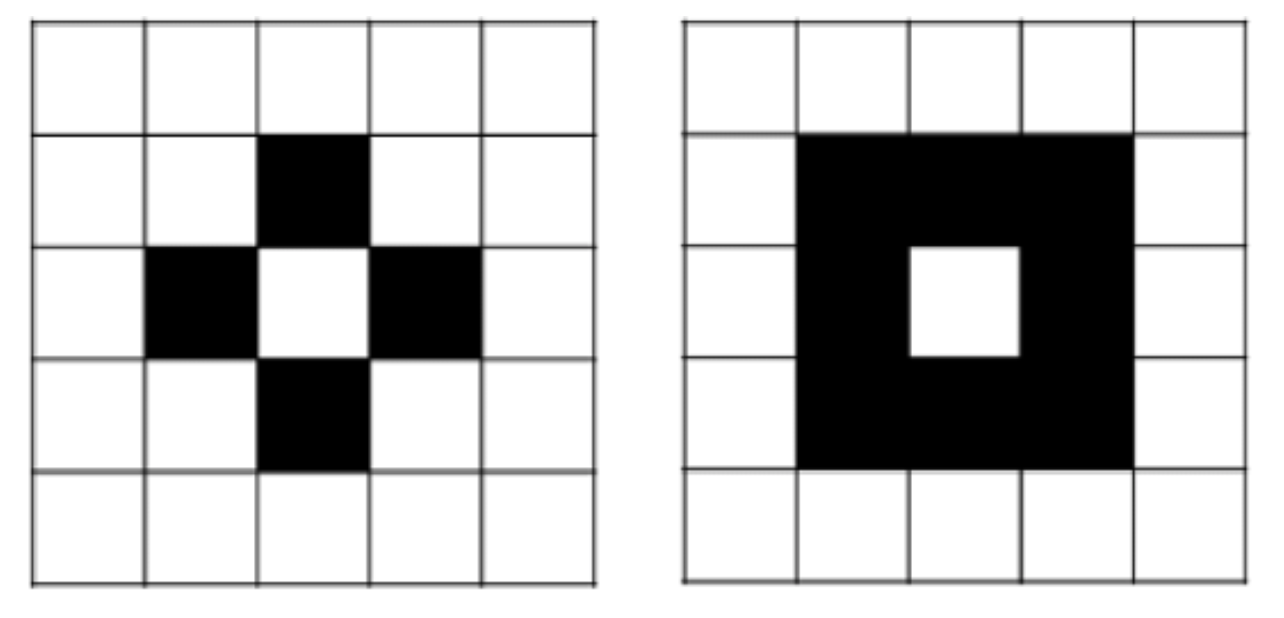
\includegraphics[width=0.5\textwidth]{Figures/von.png}\caption{Cell neighbourhoods visualised in a 2D array, neighbour cells highlighted in black. Left: the von Neumann neighbourhood. Right: the Moore neighbourhood.}\label{hoods}
\end{center}
\end{figure} 

\subsection{Modelling Wildfire}\label{Modelling_Wildfire}

A wildfire is defined as an uncontrolled fire in a rural area with combustible vegetation \cite{press2008cambridge}. Our primary objective is to recreate behaviour exhibited by wildfires for a given environment, thus describing the evolution of the fires and making accurate predictions of their future state. \newline \indent Classical methods of mathematical wildfire models include empirical and physically-based models. Empirical fire models are based on experience and intuition from past fires, while physically-based models are formulated around a fundamental conservation law of physics. For example, certain wildfire models can reproduce the relationship between the rate of fire spread and the amount of heat generated by the fires \cite{nobel_1980}, using the thermodynamic process of burning to describe the physical system of an evolving wildfire. Such classical models are often based on computationally intensive mathematics, such as hyperbolic diffusion-reaction equations \cite{1997PhRvE..56.6557M} or stochastic differential equations \cite{rothermel1972mathematical}. \newline \indent
An alternative approach to fire modelling uses a rule-based CA model with probabilistic effects. CA models are good candidates for modelling dynamical systems whose evolution depends on microscopic interactions of their constituent parts, because the interactions can be directly programmed into the rules of evolution of the cell array. The properties of CA systems are a possible representation of a wildfire system, where the fire propagation rate, fire spreading direction and the fire duration are mainly dependent on local characteristics such as vegetation, gradient and relative humidity. Cellular automaton models can incorporate these local characteristics within a theoretical fire spread mechanism, and past CA models have yielded positive results in replicating real wildfires \cite{inproceedings}.\newline \indent
Our objective is to model the 2009 Australian bushfires in the Shire of Murrindindi using cellular automata. A cell-based model is more appropriate for a simulation of this size, as finding solutions to physically-based models at the scale of $150 \times 100$ km is computationally unfeasible. The rules incorporated into our model are an adaptation of those developed by A. Aleksandridis \textit{et al.} in 2008 \cite{Aleksandridis_2008} as well as A. Quartieri \textit{et al.} in 2010 \cite{Quartieri_2010}. We incorporate the environmental factors of wind, elevation and embers into the model, and use real geographical data from the region to simulate the conditions of fire at the time of the events.

\newpage
\section{Methodology}\label{methodology}

\subsection{CA-Based Fire Model}

Our wildfire model is constructed using a two-dimensional $m$-by-$n$ matrix, corresponding to $m\times n$ individual square cells. Each cell in the matrix has an assigned integer value representing its state, with definitions shown in Table \ref{table:cellstates}:

\begin{table}[h!]
    \centering
    \begin{tabular}{|c|c|}
    \hline
     \textbf{Cell Value} & \textbf{Cell State} \\ \hline
     0 & Cell is flammable, corresponds to vegetation\\ \hline
     1 & Cell is not flammable, corresponds to bare terrain and water\\ \hline
     2 & Cell is on fire, will keep burning for a fixed amount of time\\ \hline
     3 & Cell is burnt, corresponds to a fire that has stopped burning\\ \hline
    \end{tabular}
    \caption{Cell values and their meanings used in fire simulation}
    \label{table:cellstates}
\end{table}

\noindent We define a matrix of cell values to simplify the simulated system into an array of four possible states: vegetation, non-flammable terrain, fire and burnt fuel. This matrix evolves in discrete time steps through a set of fixed rules as specified in Section \ref{ruleset}, representing the time evolution of the fire system.

\subsection{Rules for Evolution}\label{ruleset}

The simulation is performed by calculating the cell array for $N$ time steps, where the future value of each cell is determined by the current state of a neighbourhood, comprised of the given cell and a fixed number of cells in its proximity. Our method uses the 9-cell Moore neighbourhood, which balances computation speed with physical accuracy \cite{Wolfram_2002}. The rules of evolution for each discrete state from 0 to 4 are presented in Table \ref{table:futurestate}:

\begin{table}[h!]
    \centering
    \begin{tabular}{|c|c|}
    \hline
     \textbf{Current State ($t=t_0$)} & \textbf{Future State ($t=t_0+1$)}\\ \hline
     0 & 0 OR 2\\ \hline
     1 & 1\\ \hline
     2 & 2 OR 3\\ \hline
     3 & 3\\ \hline
    \end{tabular}
    \caption{Rules of fire evolution in cell array for discrete states 0 to 3}
    \label{table:futurestate}
\end{table}

\noindent Our model assumes that a fuel cell has a finite probability of catching fire, depending on the exact configuration of its neighbourhood. Fuel cells ignite with a probability $P(0\xrightarrow{}2)=p$, and remain intact with a probability $P(0\xrightarrow{}0) = 1- p$. If a cell is on fire, it will remain on fire until a specific amount of time steps has passed, determined by the fire duration $\Delta t$. The state of a non-flammable cell is static over time, remaining non-flammable for the entire simulation. Likewise, a cell that is burnt remains burnt for the duration of the simulation. To model the physical environment of fire, we calculate the probability of ignition $p$ using specified environmental variables as described in Section \ref{factors}.
\subsection{Environmental Factors}\label{factors}
The spread of fire is influenced by a sizeable number of physical factors, most determined by the exact geographical conditions at the time of fire. To create a simulation with non-trivial predictive power without requiring an unfeasible amount of computational power, our model is restricted to four major variables: elevation, wind speed, wind direction and spotting\footnote{Spotting is the phenomenon by which sparks or embers from an active fire are carried by wind to start new fires}. We define the ignition probability $p$ of a fuel cell $C$ as a function of individual probability factors $p_e$, $p_w$ and $p_s$, for elevation, wind and spotting respectively. The resulting probability of ignition $p$ is defined by:

\begin{equation}\label{netp}
    p = \begin{cases} \sqrt{p_e p_w}, & \mbox{if } C \mbox{ has neighbours on fire} \\ p_s, & \mbox{otherwise}
     \end{cases}
\end{equation}

\noindent where the square root appears for normalisation. To simplify the calculations we assume that the probability of ignition due to a cell's immediate neighbours is much larger than ignition due to spotting, $\sqrt{p_e p_w}\gg p_s$, allowing us to treat the two cases as independent. This simplifies the model and improves computation speed at the marginal loss of accuracy.\newline
\indent To calculate the elevation probability $p_e$, we use a relation derived by D. Weise \textit{et al.} in 1998 \cite{Weise_1998}. Observations show that fire has a greater rate of spread when travelling uphill compared to that of fire travelling downhill. This can be modelled using an exponential function of the elevation angle $\theta$. The elevation ignition probability $p_e$ is defined by:

\begin{equation}\label{p_elevation}
    p_e = C_1\times\sum_{i=1}^8\exp(\alpha\theta_i)
\end{equation}

\noindent where $\alpha$ is a strength parameter determining how strongly the gradient angle $\theta$ affects the ignition probability for each cell in the Moore neighbourhood for $i = 1,...,8$, and $C_1$ is a normalisation constant. For the value $\alpha=0$, the elevation change has no effect on ignition probability, and for $\alpha > 0$ the elevation has an increasing effect. The gradient angle $\theta$ is calculated using the relation:

\begin{equation}\label{theta_elevation}
        \theta = \begin{cases} \arctan{\left(\frac{h_1 - h_2}{d}\right)}, & \mbox{for adjacent cells} \\ \arctan{\left(\frac{h_1 - h_2}{\sqrt{2}d}\right)}, & \mbox{for diagonal cells}
     \end{cases}
\end{equation}

\noindent where $h_1$ is the height of the centre cell, $h_2$ is the height of the neighbour cell, and $d$ is the width of a cell in the array. Due to the square grid, a factor of $\sqrt{2}$ is included for diagonal cells. \newline \indent The effect of wind is implemented using a similar relationship, based on an exponential dependence between fire transition probability and the angle normal to the wind direction. We use a modification of the method developed by A. Aleksandridis \textit{et al.} in their 2008 paper \cite{Aleksandridis_2008}, and calculate the transition probability of fire $p_w$ to a specific fuel cell using:
\begin{equation} \label{p_wind}
    p_w = C_2 \times \sum_{i=1}^{8}\exp(\beta \times \mathbf{w} \cdot \mathbf{r}_i)
\end{equation}

\noindent where we take the sum for all neighbour cells with indices $i = 1,...,8$, $\beta$ is a wind strength parameter, $\mathbf{w}$ is the wind velocity vector, $\mathbf{r}_i$ is the direction from the middle cell to the neighbour cell $i$, and $C_2$ is a normalisation constant. The parameter $\beta$ determines the degree to which wind affects the fire transition probability, where $\beta=0$ means the wind has no effect on fire transition and $\beta>0$ has an increasing effect.\newline
\indent The third environmental factor we implement is spotting, and it affects all fuel cells in the cell array. We develop a novel method of simulating the diffusion-type behaviour of flying embers through a Gaussian convolution process, allowing us to describe the spotting phenomenon via a probabilistic approach. An example of a possible ember distribution is presented in Figure \ref{fig:emberFig}, where the heat map displays the concentration of embers in each cell before and after Gaussian convolution.

\begin{figure}[h]
\centering
    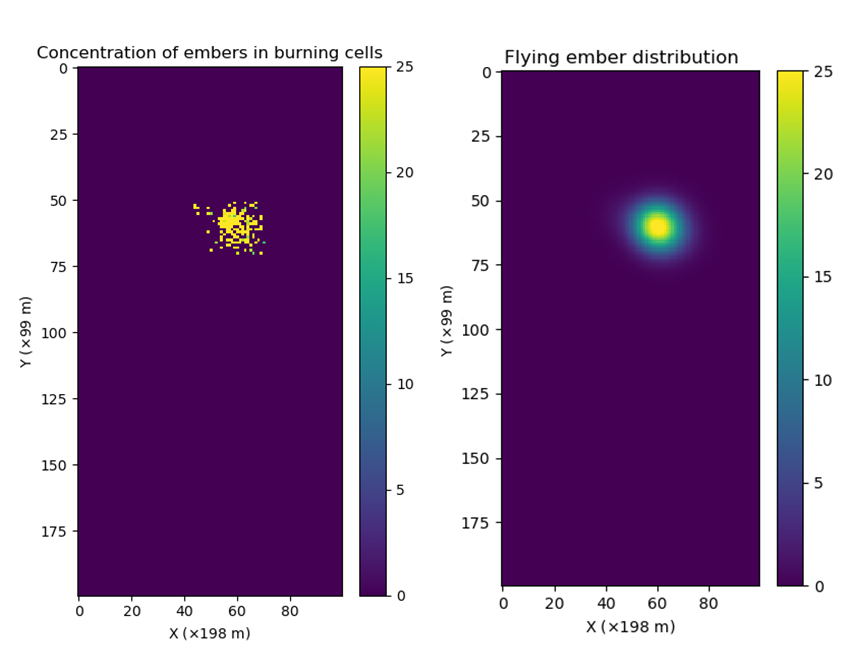
\includegraphics[width=0.95\textwidth]{Figures/embers_comp.png}
    \caption{Left: initial distribution of embers emitted by each burning cell. Right: final distribution of embers after applying Gaussian convolution. Heat map range: from 0 embers per cell (purple) to 25 embers per cell (yellow).}
    \label{fig:emberFig}
\end{figure}

\noindent  The final distribution represents the probability that an ember has landed on a given cell, thus allowing us to calculate the ignition probability $p_s$ of a fuel cell due to spotting. To obtain this distribution, we assume that each burning cell emits on average a number $E$ embers carried by wind. This process is described by a  Poisson distribution with a mean value $E$, where we pick a random value from the distribution to represent the embers emitted by each cell at each time step. The embers are carried by wind, and their spread across the landscape is modelled using a Gaussian convolution kernel with a radius $R$ given by:
\begin{equation}\label{convolution}
    R = t_{f}\times \abs{\mathbf{w}}
\end{equation}
where $t_f$ is the time that an ember remains on fire in the air, and $\mathbf{w}$ is the wind velocity vector. To ensure that the kernels travel along the direction of the wind, this process is performed along the wind vector for a length $R$. To obtain the ember ignition probability, we assume that each fuel cell has an associated normal distribution representing the number of embers required to ignite a fire in the cell. The mean and standard deviation of this distribution are defined as $M$ and $\sigma$ respectively. We obtain a relationship for the ignition probability of any cell due to the spotting effect, denoted by $p_s$:

\begin{equation}\label{p_spotting}
    p_s(x) = \frac{1}{2}\left[1 + \erf\left(\frac{x-M}{\sigma \sqrt{2}}\right)\right]\\
\end{equation}

\noindent where $\erf$ is the Gauss error function, and $x$ is the number of embers that have landed on the cell after the convolution process. To simplify the computational requirements of this calculation, we defined a discrete range of $x$-values for which the ignition probability is calculated. We define $p_s(x)$ such that $p_s(M+3\sigma) \approx 1$, and $p_s(M-3\sigma) \approx 0$, and the values of $x$ within these limits are rounded to the nearest decimal point. This trade-off sacrifices marginal accuracy for a substantial computational speed gain. \newline
\indent In addition to incorporating these environmental effects, the model can also use a simple alternative rule set. To do this, the cellular automaton in our code can be defined such that the ignition probability $p$ of a fuel cell $C$ at index $i$ in the array is given by:
\begin{equation}\label{p_ignition}
    p = \frac{1}{8} \times \sum_{i=1}^8 C(i) \delta_{C(i),2}
\end{equation}
where the index $i = 1,...,8$ belongs to the Moore neighbourhood of the cell $C$, a cell on fire is represented by $C(i)=2$ and $\delta$ is the Kronecker delta function. This expression gives us the simple relation $p=F/8$, where $F$ is the number of neighbouring cells on fire. To revert to this calculation for the ignition probabilities, the elevation and wind strength parameters are normalised. This means that for an arbitrary wind and elevation input, if $\alpha,\beta=0$ then the ignition probability $p$ is calculated according to Equation \ref{p_ignition}.

\subsection{Simulation Environment}

We use Python v3.7.4 as our main simulation environment, with Numpy v1.17 and Scipy v1.4.1 as additional packages. The source data for vegetation, wind and elevation is processed using MATLAB R2019b with the Mapping Toolbox\texttrademark{} and the Image Processing Toolbox\texttrademark{}. An overview of the Python code is given as a class diagram in Appendix \ref{code}, and the source data is acquired through Geoscience Australia's Web Portal \cite{Geodata}.

\newpage
\section{Results Part I: Fire Model Analysis}\label{results_1}

We use our cellular automata model to simulate the progression of wildfire spread under a variety of conditions and quantify the effect of introducing different parameters into the model. These parameters include the introduction of embers, wind and elevation. In Section \ref{4.1} we analyse how the fire front and rate of spread are depend on the fire duration $\Delta t$ without any of these environmental parameters added. We also analyse how the distribution of the final percentage of burnt cells varies across many simulations. Then, in Section \ref{4.2} we analyse how the introduction of elevation affects the behaviour of the simulated fire and at what point the elevation in a system becomes dominant. Section \ref{4.3} analyses how the introduction of wind into the simulation affects the direction of the fire and the rate of fire spread, and Section \ref{4.4} analyses the introduction of embers into the system and how this affects the fire behaviour. In Section \ref{4.5} we analyse how the probability of ignition is dependent on all the aforementioned environmental parameters, formulating numerical equations for fire spreading in Section \ref{numericalfire}. Finally, in Section \ref{modellimits} we discuss the limitations associated with this model.

\subsection{Fire Front and Rate of Spread}\label{4.1}
To analyse how the fire front is affected by the value of the fire duration $\Delta t$, we create a simulation with a 100$\times$100 grid of flammable cells. In the centre of the grid, we start $5\times5$ fire cells with no additional environmental factors added. The simulation is run with the following initial values: the fire duration $\Delta t$ is varied between the values $1,2,3,4,5$, and the procss is iterated for $N=50$ time steps. In Figure \ref{f41} we display the end result of three of these simulations.

\begin{figure}[H]
\centering
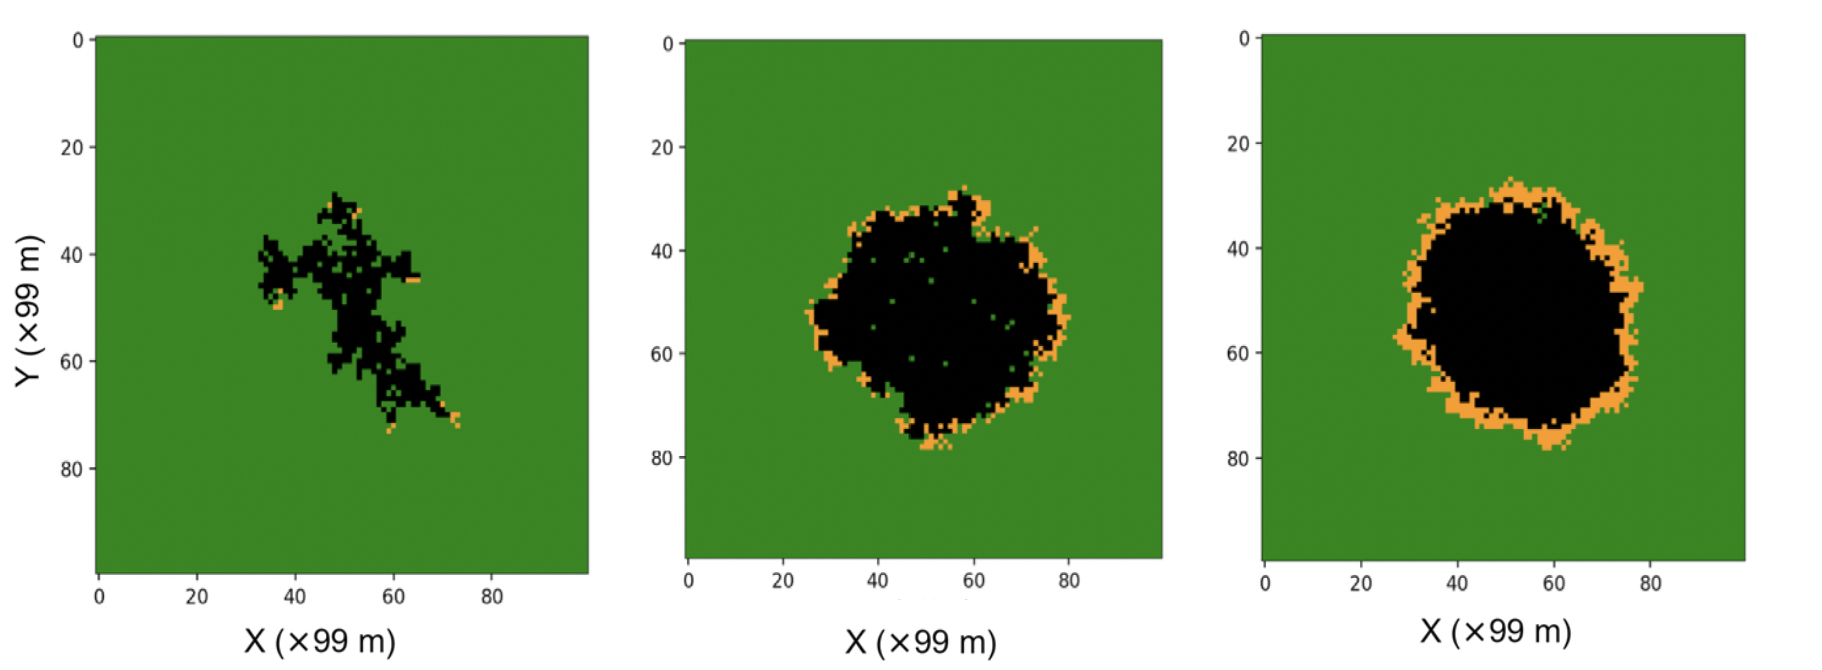
\includegraphics[width=\textwidth]{Figures/abba.png}
\caption{Left: Automaton with $\Delta t = 1$ after $N=50$ steps. Middle: Automaton with $\Delta t = 3$ after $N=50$ steps. Right: Automaton with $\Delta t = 5$ after $N=50$ steps. Colour code: \newline green = fuel cells, orange = fire cells, black = burnt cells.}
\label{f41}
\end{figure}
\newpage

\noindent We observe that with $\Delta t=1$ the fire behaviour is very sporadic and unpredictable. To obtain a measure of uncertainty in the evolution of the system, each simulation is repeated $5$ times. Across the different runs, the fire moves in random directions and does not have any overall net movement in a particular direction. \newline \indent For $\Delta t=2$, the final percentage of burnt cells after the simulation is equal to $14.36\pm2\%$, resulting in a fire spreading rate of 14.36 cells per $N$. With $\Delta t=3$ we observe that the spread of fire is more radially uniform, and for $\Delta t=5$ the fire front is thicker as there are more fire cells present. For $\Delta t=3$ the final percentage of burnt cells is equal to $38.86\pm2\%$, giving a rate of fire spread of 38.86 cells per $N$. Similarly, running the simulation for $\Delta t=5$ gives us a final percentage of burnt cells equal to $50.36\pm2\%$, corresponding to a rate of spread of $50.36$ cells per $N$. We observe that increasing $\Delta t$ from 2 to 5 results in the rate of fire spread increasing by a factor of $3.51\pm0.05$. \newline \indent The implication of these results is that the fire duration $\Delta t$ is a critically important factor when estimating the rate of spread. Applying this to real fires, our result suggests that the longer a fire is burning in one particular area, the greater the total rate of fire spread will be.\newline \indent To analyse the distribution of the percentage of burnt cells, we find the average occurrence of each value of percentage burnt. We create a simulation with a $25\times25$ grid of fuel cells and start the fire as a $5\times5$ square in the centre of the grid. The simulation is run for $N=50$ steps and we use values of $\Delta t=1,2,3$. Figures \ref{f42} and \ref{f43} show the distribution of the final percentage of burnt cells across $1000$ runs of the simulation for $\Delta t=1$ and $\Delta t=3$ respectively.

\begin{figure}[H]
\begin{center}
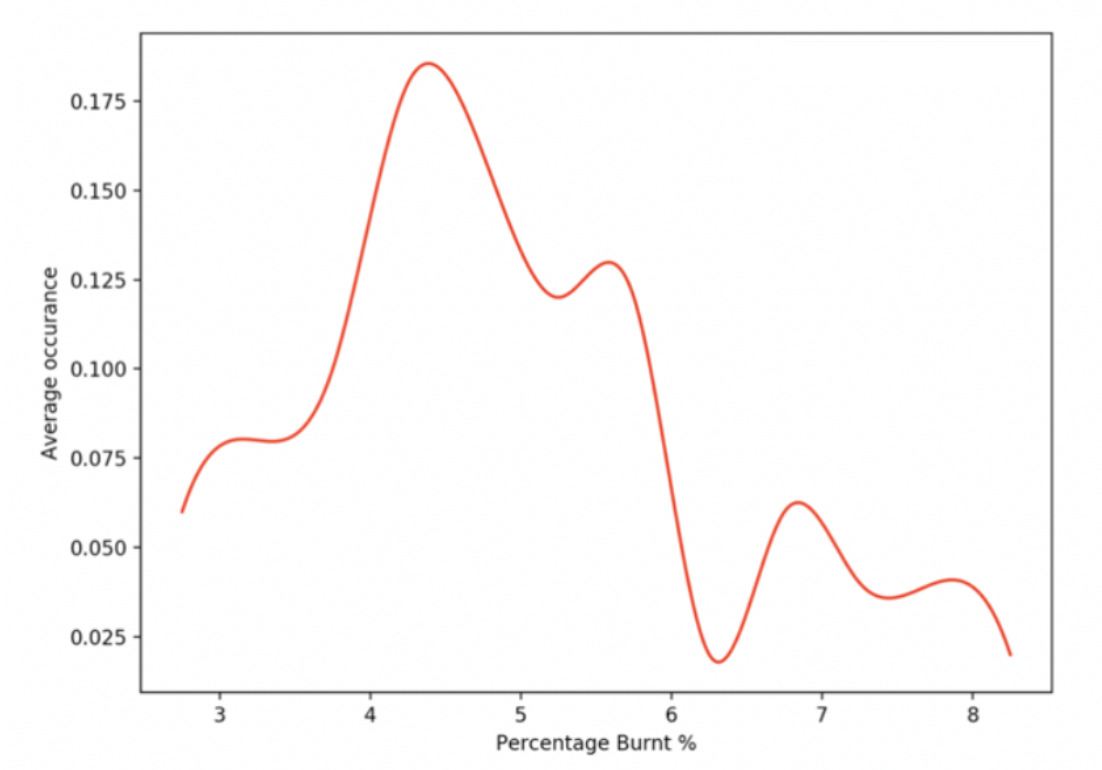
\includegraphics[width=0.9\textwidth]{Figures/ffff1.png}
\caption{Average occurrence of the percentage of burnt cells across 1000 simulations. Grid size: $(25\times 25)$ fuel cells, fire duration $\Delta t=1$, simulation duration $N=50$ time steps.} 
\label{f42}
\end{center}
\end{figure}

\begin{figure}[H]
\begin{center}
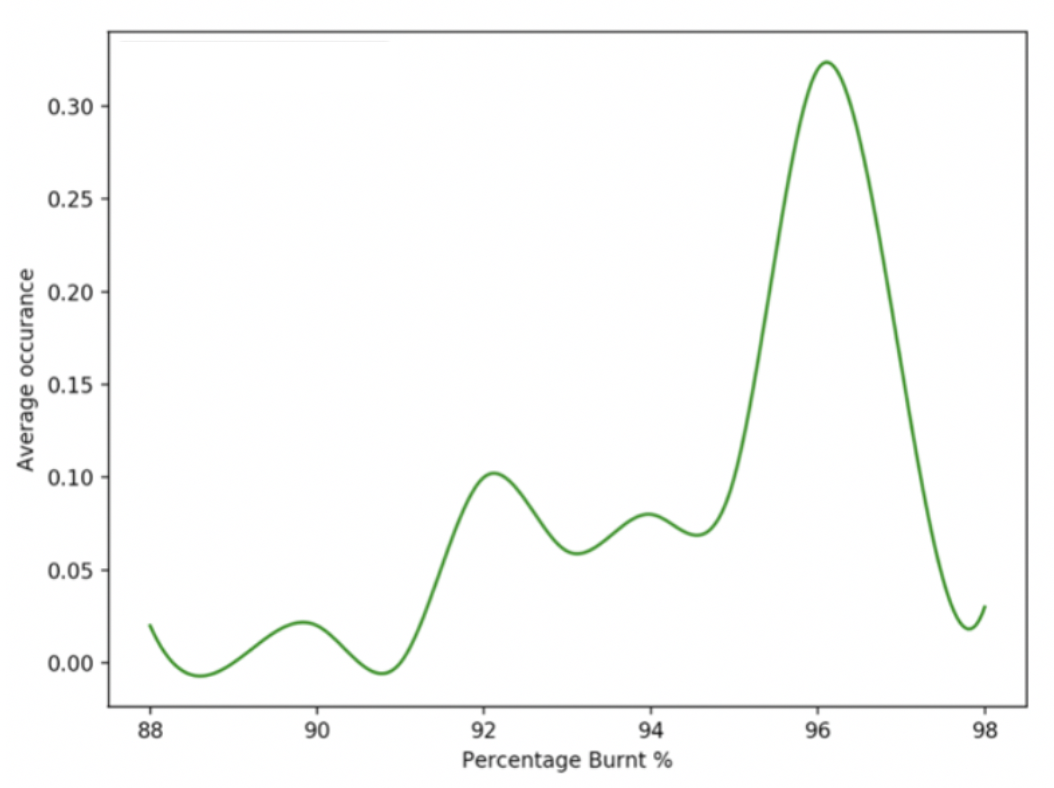
\includegraphics[width=0.9\textwidth]{Figures/ffff2.png}
\caption{Average occurrence of the percentage of burnt cells across 1000 simulations. Grid size: $(25\times 25)$ fuel cells, fire duration $\Delta t=3$, simulation duration $N=50$ time steps} 
\label{f43}
\end{center}
\end{figure}

\noindent We observe from Figures \ref{f42} and \ref{f43} that the distribution of the percentage of burnt cells for both $\Delta t=1$ and $\Delta t=3$ exhibit sporadic behaviour within the range shown. However, both distributions have a distinct peak. For $\Delta t=1$ the peak occurs at $4.25\pm0.3\%$ whilst for $\Delta t=3$ the peak occurs at $96.0\pm0.1\%$. \newline \indent The difference in these distributions shows a dramatic increasing effect that increasing the value of $\Delta t$ has on the surface area burnt by the fires. For the values $\Delta t=1,3$, the percentage of burnt cells has a narrow peak with a $\pm 2\%$ standard deviation. With $\Delta t=1$ the probability of the percentage of burnt cells being over 10\% is effectively zero, but with $\Delta t=3$ the probability of the percentage of burnt cells being under 85\% is also nearly zero. \newline \indent Interestingly, for $\Delta t=2$ the distribution of results has no distinct trends and the spread of values resembles a sinusoidal wave. For this fire duration, the values of the percentage of burnt cells range from 5\% to 80\% with no distinct peaks in the distribution. This suggests that for a fire duration of $\Delta t = 2$, the fires propagate randomly across the landscape without a uniform fire front. \newline \indent As a model of real wildfires, our simulation suggests that fire duration is a critical parameter determining the global spread of the fires across their environment. For our model to accurately represent wildfires, the precise value of $\Delta t$ needs to be determined by comparing our simulated results to real-world fires, and matching their rate of spread.

\subsection{Effects of Elevation}\label{4.2}

To analyse the effects of elevation, we investigate how the value of the strength parameter $\alpha$ affects the fire percentage of burnt cells. We create a simulation with the addition of an elevation parameter, represented by a height function $h=h(x,y)$ where $x$ and $y$ are the coordinates of each cell. Our test simulation consists of a 100$\times$100 grid of fuel cells, with 5$\times$5 fire cells at its centre, burning for a fire duration of $\Delta t = 3$. For this simulation, wind and embers are omitted, and we vary the value of $\alpha$ from $0.1$ to $0.5$ in steps of $0.1$. The elevation function used is $h(x,y)= x+y$, providing a uniform gradient. Figure \ref{f44} shows the evolution of the percentage of burnt cells in the array over time for each value of $\alpha$, for a duration of $N=100$ time steps.

\begin{figure}[H]
\begin{center}
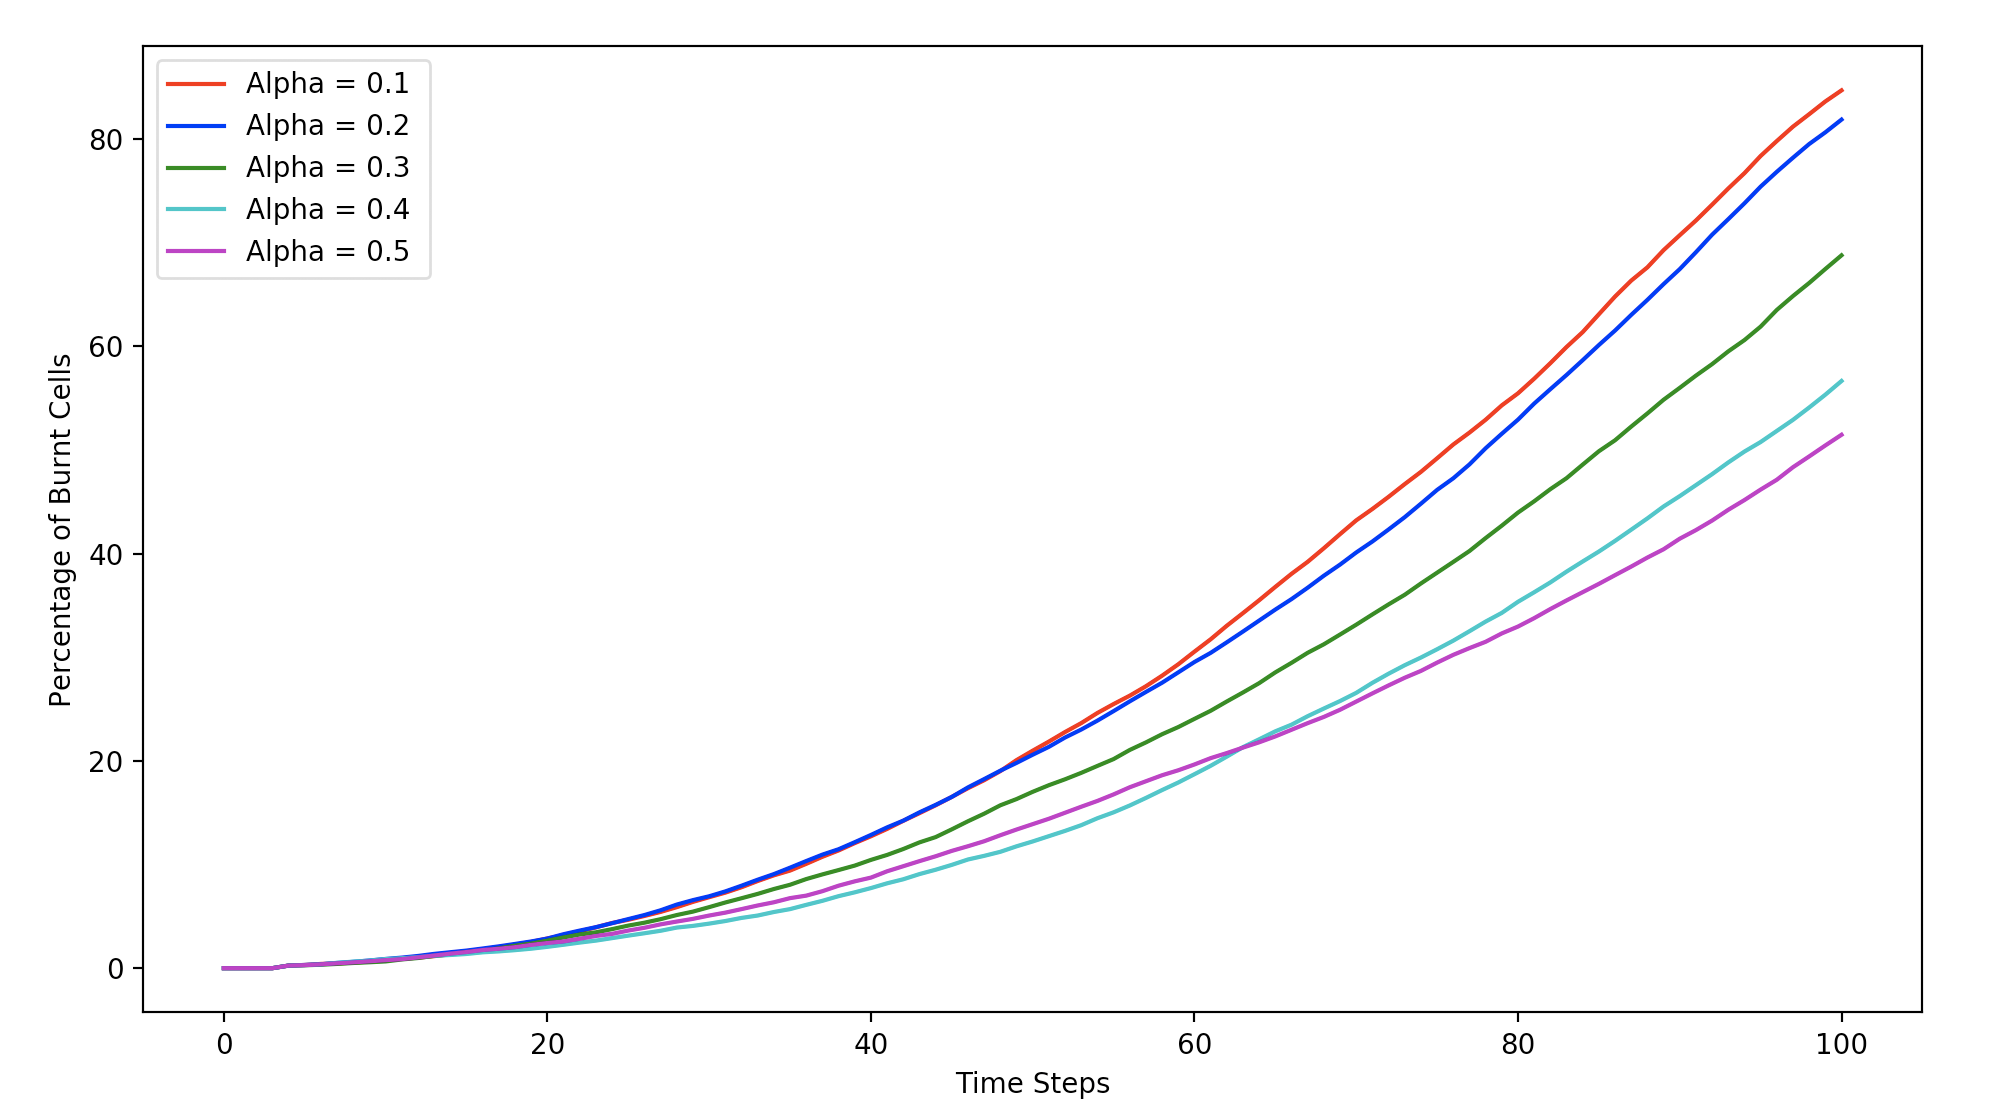
\includegraphics[width=0.9\textwidth]{Figures/f3.png}
\caption{Percentage of burnt cells for every time step $N$ with different values of $\alpha$. Initial conditions: $(5\times5)$ fire cells in the centre of a $(100\times 100)$ grid of fuel cells.} 
\label{f44}
\end{center}
\end{figure}

\noindent We observe that as $N$ increases, the number of burnt cells increases monotonically. A greater value of $\alpha$ results in a lesser rate of spread for the simulated fire. For example, when $\alpha=0.1$ the rate of spread is equal to $87.65\pm0.2$ cells per $N$ whilst for $\alpha=0.5$ the rate of spread is equal to $49.03\pm0.2$ cells per $N$. By increasing the value of $\alpha$ from 0.1 to 0.5 the rate of fire spread changes by a factor $1.788\pm0.04$. This result implies that the effect of elevation reduces the overall rate of fire spread. Physically, the simulation suggests that fire is restricted by the effects of elevation, particularly large differences in elevation. We find the specific value of $\alpha$ that completely prevents fire from spreading downhill, by using the same simulation discussed in Section \ref{4.2}. We continue increasing the value of $\alpha$ until we find that the fire doesn't spread downhill at all, and obtain a result of $\alpha=1.2\pm0.05$. Physically, this implies that there is a point in the simulation when the effects of elevation are so strong that a fire would not be able to spread downhill at all.

\subsection{Effects of Wind}\label{4.3}

To find how the wind parameter affects the fire spread, we create a simulation where the effect of changing the value of $\beta$ can be seen. This simulation consists of a column of fuel cells with a width of 40 cells and height of 100 cells. We start 5$\times$5 fire cells in the centre of one end of the column so the fire can only travel down the column. The wind vector is chosen as $\mathbf{w}=(0,5)$ so the wind is directed up the column of cells. We run this simulation with values of $\beta$ ranging from 0.1 to 0.5 in steps of 0.1. Figure \ref{f45} shows how the percentage of burnt cells evolves in time for each value of $\beta$ used.

\begin{figure}[H]
\begin{center}
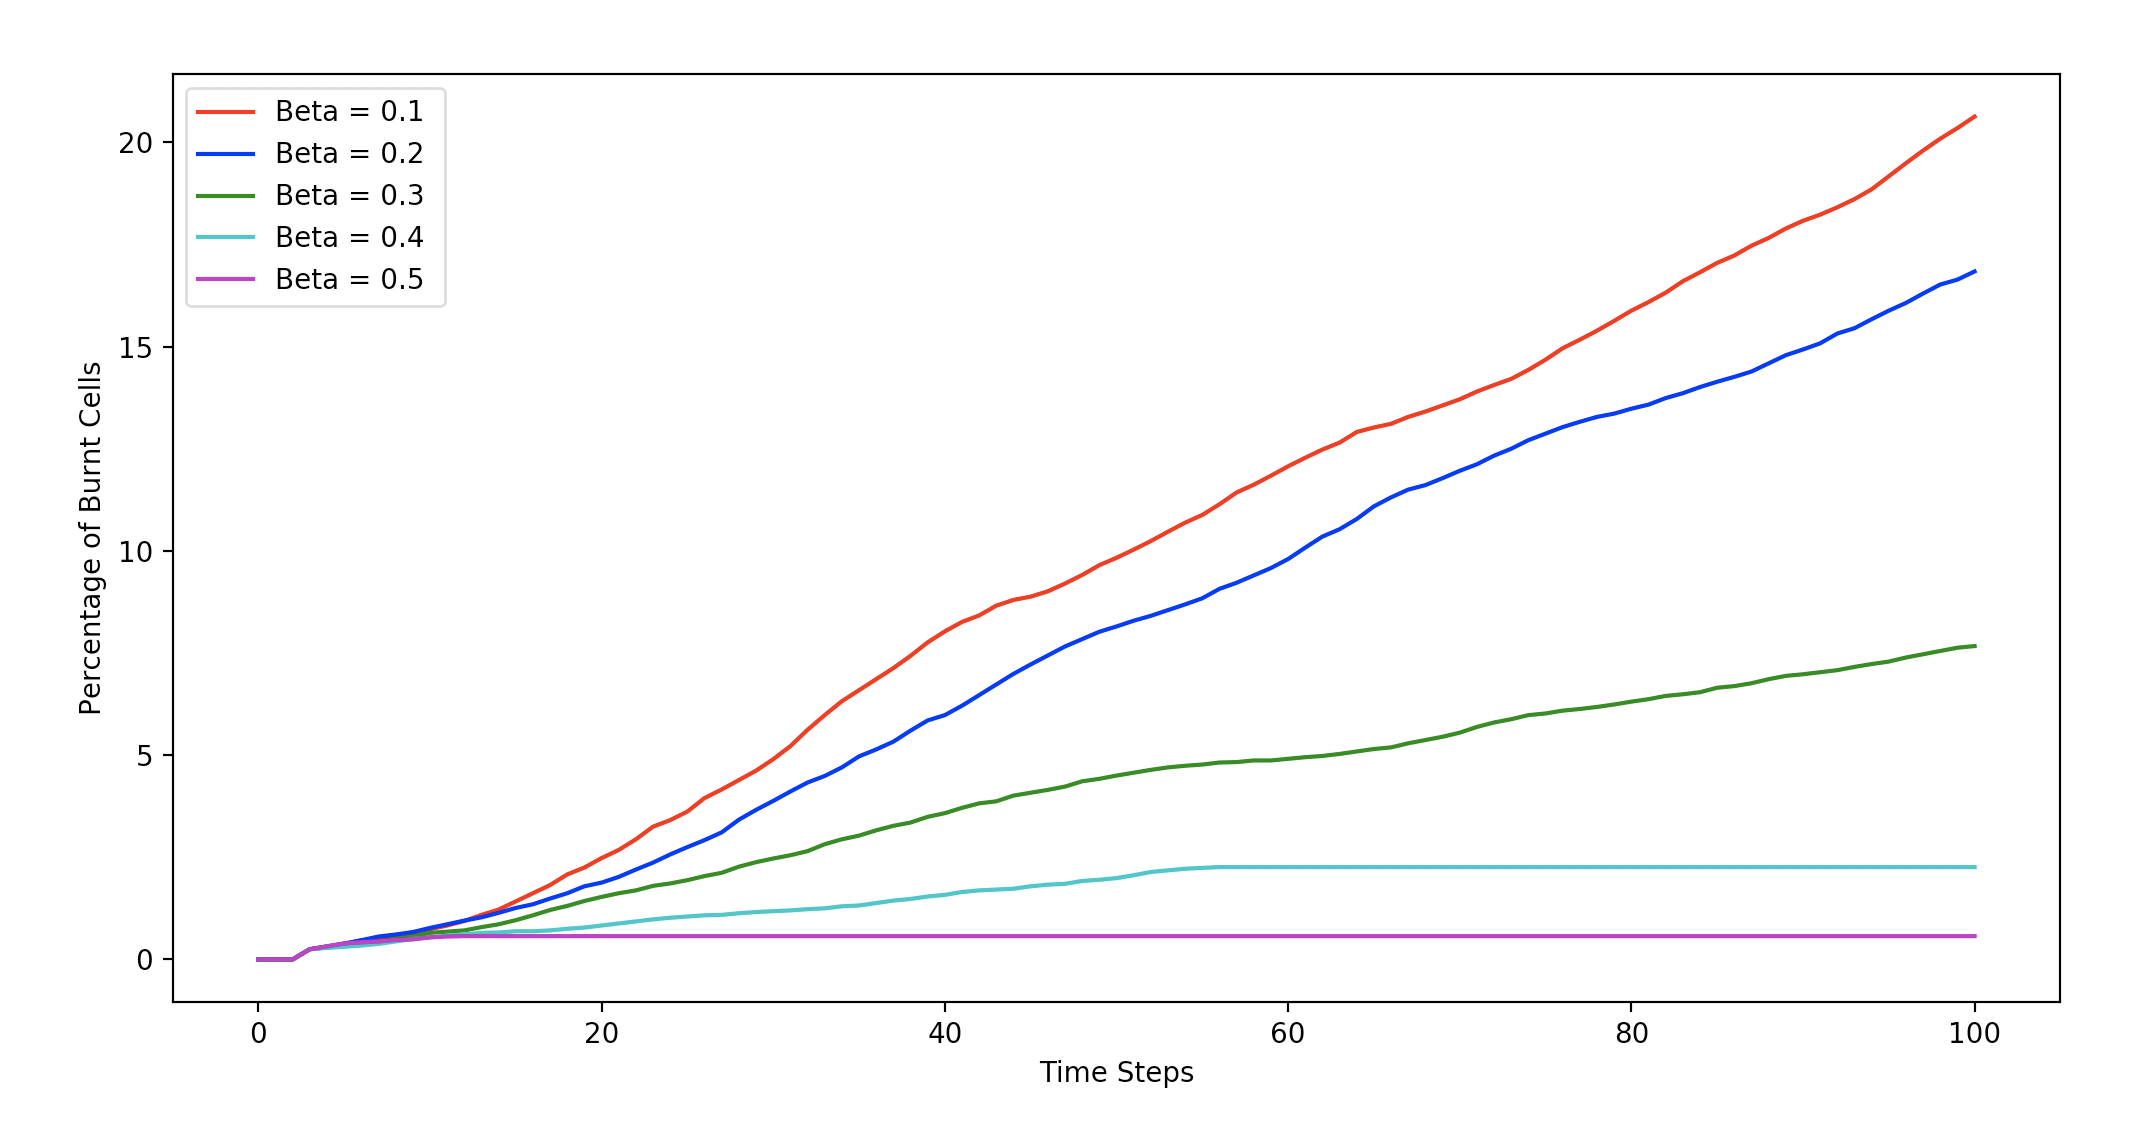
\includegraphics[width=0.9\textwidth]{Figures/f4.png}\caption{The values of percentage of burnt cells for every $N$ for different values of $\beta$} 
\label{f45}
\end{center}
\end{figure}

\noindent We observe that for a greater value of $\beta$, the percentage of burnt cells for the same $N$ is smaller. For $\beta=0.5$ we see that the fire burns out relatively quickly, extinguishing in $N \approx 10$ time steps, but for $\beta=0.1$ the percentage of burnt cells is still increasing at $N=100$. At $N=100$ and $\beta=0.5$ the percentage of burnt cells is equal to $0.57\pm0.1\%$ whereas for $\beta=0.1$ this value is equal to $20.14\pm2\%$. \newline \indent These results imply that wind blowing in the opposite direction to fire spread has a negative impact on the rate of fire spread. Physically this suggests that the danger of fire spread is considerably decreased if the wind is blowing in the opposite direction. It should be noted that the parameter $\beta$ needs to be determined via empirical analysis, comparing the effect of wind on real bushfires and our simulated results. \newline \indent To find physical limits for the parameter $\beta$, we use this simulation to find the value of $\beta$ where the fire is completely restricted by the wind. We increase the value of $\beta$ until we find that the fire does not spread at all, and observe this value to be at $\beta=0.95\pm0.05\%$. This value signals the point where the simulated strength of the wind is so great that fire travelling against the wind is effectively extinguished. To continue our analysis, we study the effect of wind blowing in the same direction as the fire spread in Section \ref{4.5}.

\subsection{Effects of Embers}\label{4.4}

Our model incorporates several parameters which relate to the introduction of embers into the system. To analyse this phenomenon we create a simulation where the number of embers $E$ released by a fire cell is varied. We create a simulation with $100\times100$ flammable cells and start $5\times5$ fire cells in its centre, with the initial parameters $\Delta t=2$, $t_f=10$, $M=5$, $\sigma=2$. The number of embers emitted from a cell are varied between the values $E=3,4,5,6,7$. Figure \ref{f46} shows how the percentage of burnt cells increases with time for each of these values. 

\begin{figure}[H]
\begin{center}
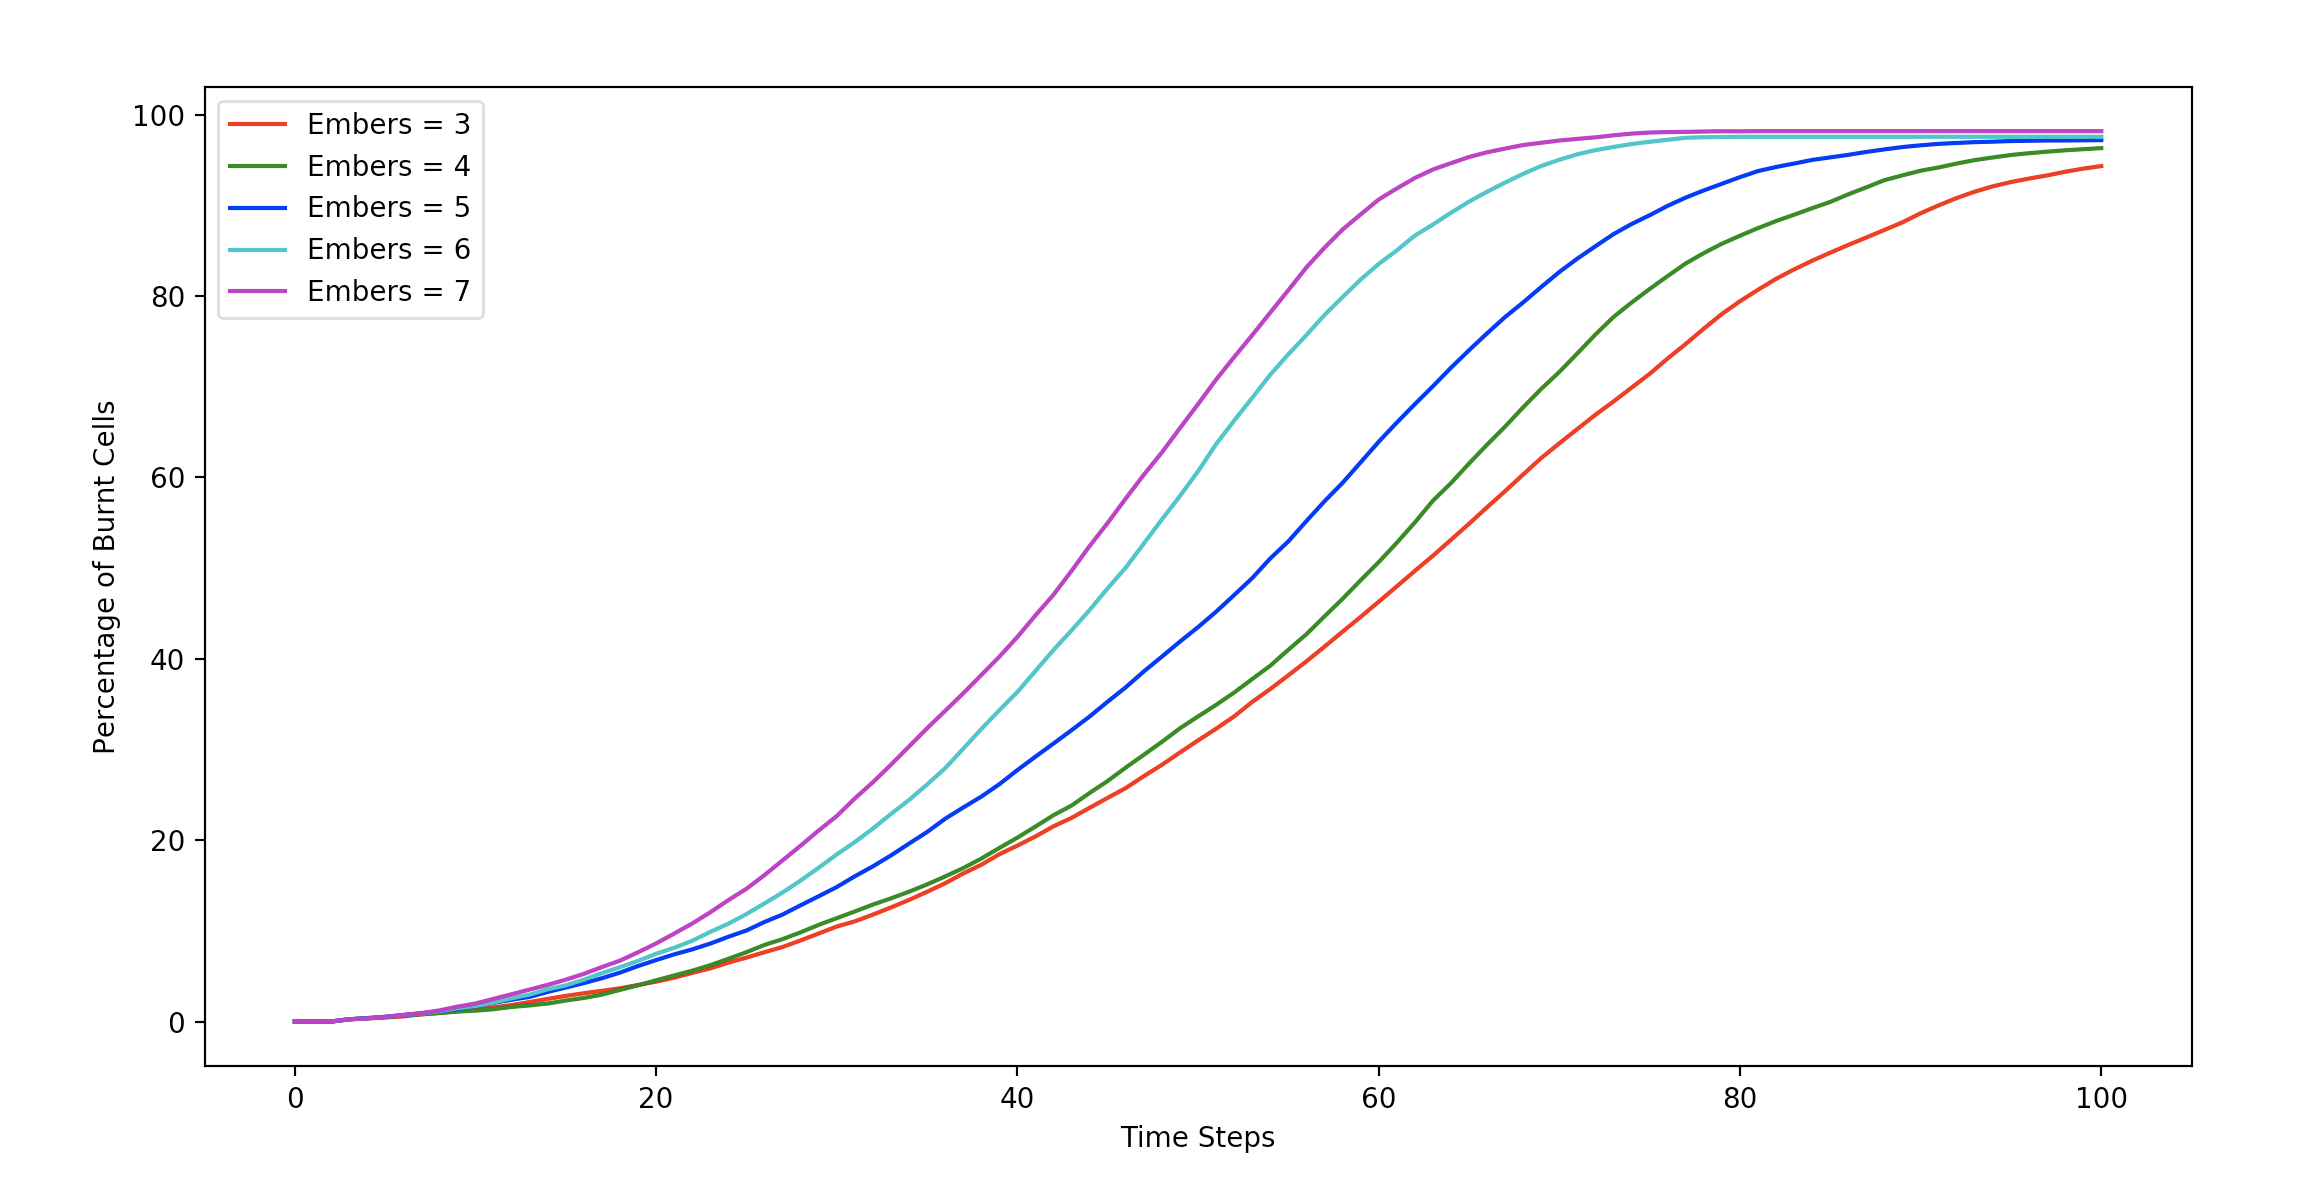
\includegraphics[width=0.9\textwidth]{Figures/f5.png}
\caption{The values of percentage of burnt cells for every N for different values of E.} 
\label{f46}
\end{center}
\end{figure}

\noindent We observe that the introduction of embers has a dramatic effect on the rate of fire spread and that a larger number of embers results in a greater percentage of burnt cells at every time step. For example, when $E=3$ the rate of fire spread is equal to $94.53\pm2$ cells per $N$. We recall from Section \ref{4.1} that without any additional environmental parameters the rate of fire spread for $\Delta t=2$ is equal to 14.36 cells per $N$. This implies that by introducing embers into the simulation the rate of fire spread increases by at least a factor of $6.583\pm2$. Using this result we infer that one of the primary methods of fire transition is through the embers emitted by a fire. Without the spreading of embers, fires would be much more contained.

\subsection{Fuel Ignition Probability}\label{4.5}

To further understand the effect which each environmental aspect of model has on the simulated fire spread, we analyse how the probability of ignition of a cell changes with the addition of different parameters and obstacles. We perform a simulation with a 50$\times$50 grid of fuel cells with 5$\times$5 initial fire cells in the top left corner. The simulation is run for N=200 steps with $\Delta t=2$. To obtain the fuel ignition probability, the average result for each cell is calculated across 1000 runs with identical initial conditions. Figure \ref{f47} shows two probability heat maps; one for this simulation with no additional parameters and one for a simulation with a $30\times30$ block of non-flammable cells in the centre of the grid.

\begin{figure}[h!]
\begin{center}
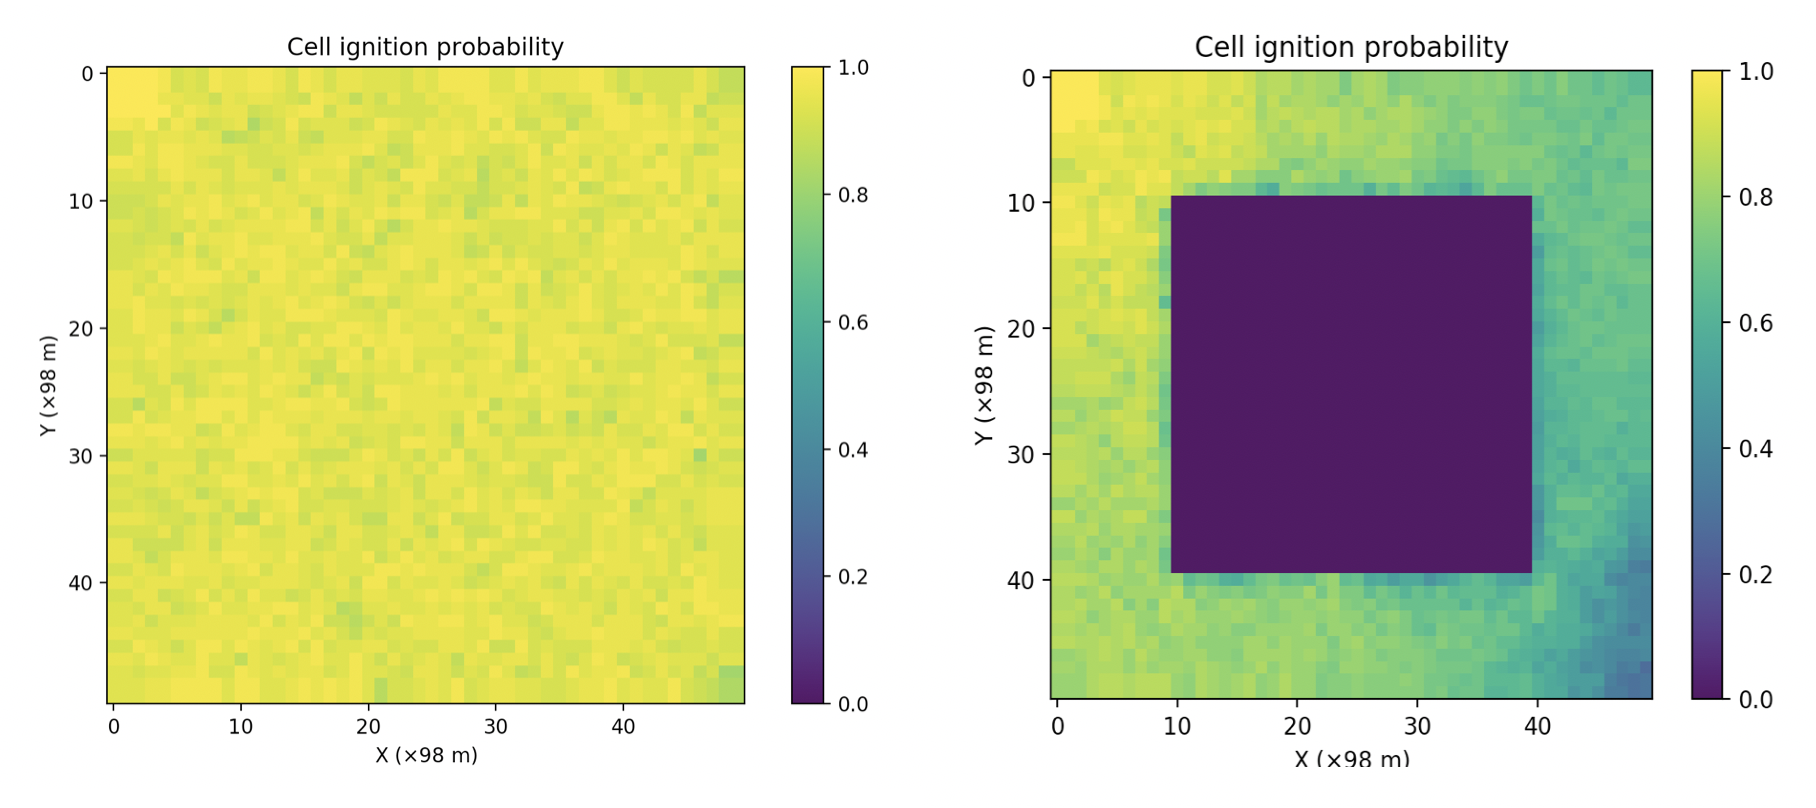
\includegraphics[width=0.8\textwidth]{Figures/h.png}
\caption{Probability heat maps of ignition. Left: result of simulation without any wind, elevation, embers or obstacles added. Right: result of identical simulation with a $30\times30$ block of non-flammable cells added at the centre.}\label{f47} \end{center}
\end{figure} 

\noindent We compare the two results by investigating the probability of ignition of the cell in the bottom right corner, located opposite to the starting fire at position $(49,49)$. In the absence of obstacles, the probability of ignition for this cell is equal to $0.84$, and in the presence of a $30 \times 30$ block of non-flammable material, this probability decreases to $0.32$. We repeat the same process with the addition of elevation, using $\alpha = 0.3$ and an elevation function $h(x,y) = 100+\sin(\frac{x}{10})+ 20\cos(\frac{y}{100})$. For these conditions, without the presence of the non-flammable cells the probability of ignition of the corner cell is $0.08$. With the block of non-flammable cells included, the probability of ignition is equal to $0.01$.\newline
\indent We repeat the procedure with the addition of wind, using a wind vector $\mathbf{w}=(5,-5)$ and $\beta=0.3$. The probability of ignition with these conditions, without the block of non-flammable cells is equal to $0.99$, and the probability of ignition with the block is $0.88$. We then calculate the ignition probability of the cell at $(49,49)$ with the addition of embers, with the following conditions: $E=10$, $M=10$, $t_f=5$ and $\sigma=2$. In the scenario without the block of non-flammable cells, the probability of ignition is equal to $0.96$, whereas in the presence of the block the ignition probability is $0.92$. We observe that when the effects of embers are taken into account the probability of ignition increases by a factor of 1.14$\pm0.01$. If both elevation and embers are taken into account, then the probability of ignition decreases by a factor of  10.5$\pm0.5$. \newline \indent We concur from these results that if wind is blowing in the direction of a cell, then the probability of ignition to that cell is greater by a factor of $1.20\pm0.01$. Physically this suggests that the most dangerous place to be in relation to a fire is directly in line with the direction of the wind. Our simulation implies that to reduce the probability of a wildfire reaching a particular location, the number of nearby non-flammable obstacles should be increased. \newpage 
\subsection{Numerical Fire Equations}\label{numericalfire}
We use our fire simulation to find a set of equations that describe the probability of ignition of a particular cell. We determine the relationships between the probability of ignition $P$ and the following variables: the  number of time steps $T$ the fire has been spreading for since the fire started, the distance $X$ between a selected cell and the nearest fire cell at the start of the simulation, the value of $\beta$. We create a simulation consisting of a single fire cell with $\Delta t = 2$  at the centre of a $30\times30$ grid of fuel cells, running for $N=20$ time steps. No elevation, wind or embers are included for simplicity.  Figure \ref{f48} shows the resulting ignition probability heat map after 1000 runs.

\begin{figure}[h!]
\begin{center}
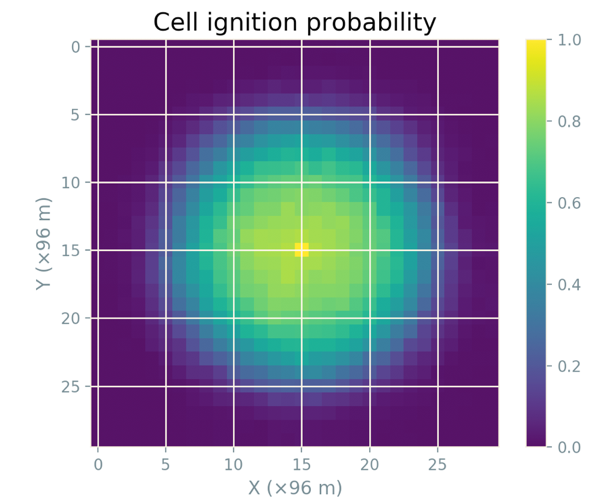
\includegraphics[scale=0.5]{Figures/h5.png}
\caption{Ignition probability heat map for a simulation with a single initial fire cell in the middle of $30\times30$ fuel cells, after $N=20$ steps.} 
\label{f48}
\end{center}
\end{figure} 

\noindent We observe that the probability of ignition $P$ of a given cell decreases with distance from the starting fire, following an approximate power law. The exact relationship is determined in conjunction with the dependence of $P$ on the number of time steps $N$ for which the simulation is run for. We run the same simulation used to create Figure \ref{f48} while varying the number of steps $T$ the simulation is run for. To obtain numerical values in this relationship, we generate a large number of identical simulations and obtain power law fittings between $P$ and the parameters $X,T$ and $\beta$. The resulting equation combines all of these parameters, giving us a function $P(T,X,\beta)$:

\begin{equation}
    \large
    P(T,X,\beta) = \begin{cases}\chi_1 \frac{T^{2.049} \beta^{1.598}}{X^{0.2017}} + \chi_2 \pm 0.1464& \mbox{\normalsize when wind blows toward the cell}\\
    \chi_3 \frac{T^{2.049}} {X^{0.2017} \beta^{2.243}} + \chi_4 + \pm 0.1964& \mbox{\normalsize when wind blows away from the cell}
    \end{cases}
    \label{p2}
\end{equation}

\noindent where the constants $\chi_1 = 5.69 \pm0.05\times 10^{-4}$, $\chi_2=0.577\pm 0.05$,$\chi_3=8.04\pm0.2\times 10^{-8},$ and $\chi_4=0.212\pm0.05$. Equation \ref{p2} can be used to estimate the probability of ignition for a simulation of size $30 \times 30$ grid with a single fire cell of $\Delta t=2$ at the centre of the grid, assuming the following conditions are satisfied: $T>20$ and $0.05<\beta<0.1$. \newline 
\indent We find that for a very large value of $T$ or a very low value of $X$ the probability of ignition is very close to 1. This implies that in such conditions it is effectively guaranteed that the fire will ignite a particular cell. Moreover, we can see that the relationship between the probability of ignition and the strength of wind is very dependent on the direction of the wind. In terms of real wildfires, we postulate that the areas with the lowest chances of ignition need to be far away from the fire and in a direction where the wind is blowing away from the fire.

\subsection{Limits of the Fire Model}\label{modellimits}

We have observed how our model replicates wildfire behaviour with the effects of different environmental parameters. We demonstrate that elevation, wind and spotting can all be incorporated into the cellular automaton simulation with physically sound results, showing that our methodology is a valid starting point for a wildfire simulation. \newline \indent The central limitation of our model is in determining the exact values of the fire parameter $\Delta t$ and environmental strength parameters $\alpha, \beta, E,M,t_f$ and $\sigma$. We observe a dramatic change in fire behaviour depending on the value of $\Delta t$, where the difference between $\Delta t=1$ and $\Delta t=3$ changes the eventual area burnt by fire by $80\%$. To model fire in a particular situation, we require knowledge of which value of $\Delta t$ is physically accurate. Obtaining this information requires a large amount of precise historical data and may prove challenging. Likewise, without knowing appropriate values of $\alpha$ and $\beta$ the model cannot be expected to accurately reproduce real fire behaviour. \newline \indent Furthermore, the environmental parameters within our model do not always yield physical results. For example, if we set $\alpha>4.0$ or $\beta>4.0$ in a simulation, then the fire model shows all fire being instantly extinguished, with no spread in any direction. Another non-physical result can be obtained by configuring the ember parameters $E,M,t_f$ and $\sigma$. There exists a critical point where the effects of embers become so large that the fire behaviour becomes explosive and extremely non-physical, spreading across the map with increasing speed until all fuel has been burned. This explosive behaviour causes the rate of fire spread to reach values of over 500 cells per $N$, depending on the values of the ember variables used. When $t_f=10$ and $\sigma=2$, the critical point occurs at $E=3M$.\newline \indent As an additional remark, the rules used within this automaton are probabilistic and do not consider the complex physics behind fire transitions. Hence there is no guarantee that these rules will realistically model fire or preserve quantities that have associated conservation laws such as energy or momentum. To obtain a picture of the true physical accuracy of our model, we compare data produced by the cellular automaton model with data from real bushfires. This is the subject of Section \ref{results_2}.

\newpage

\section{Results Part II: Case Study of Murrindindi Fire}\label{results_2}

\subsection{Historical Context}

In order to analyse the predictive power of our simulation, we perform a case study of the 2009 Australian Bushfires in the region of Murrindindi, Victoria. Our interest is to simulate the events known as the "Black Saturday bushfires" in the region and recreate the evolution of these fires using our cellular automaton model. Our aim is to quantify how well our simplified system predicts aspects of fire behaviour when working on the scale of tens of kilometers, and investigate if the real events differ from the predictions of our model.\newline
\indent Starting on February 7\textsuperscript{th}, 2009, a series of bushfires burnt over $450,000$ hectares of land and caused 173 fatalities in a series of events now referred to as the Black Saturday bushfires \cite{RoyalCommission}. The conditions at the time were ideal for a catastrophic wildfire event: Southeastern Australia had suffered from a prolonged period of low humidity and temperatures of over $45\degree$C. On Saturday 7\textsuperscript{th} at 14:55, a fire of unknown origin started in Northern Murrindindi, and it quickly spread across the landscape. Over the course of the day, the ensuing wildfire destroyed over 500 houses and resulted in the deaths of 39 people in the area of Marysville.
\subsection{Initial Conditions for Simulation}
\indent To simulate these events, geographical data including elevation and vegetation maps is obtained from the web portal for the Geoscience Department of the Australian Government \cite{Geodata}. A rectangular map spanning the coordinates  $(38.00 -37.00)$\degree S, $(145.50 - 147.00)$\degree E is used as an input for the simulation. The fire modelling array is overlaid on top of elevation data, and the simulation uses the vegetation map as its initial state. A colour-coded relief map is presented in Figure \ref{topography}, and the forest coverage of the same region is displayed in Figure \ref{forestcover}.

\begin{figure}[h!]
\centering
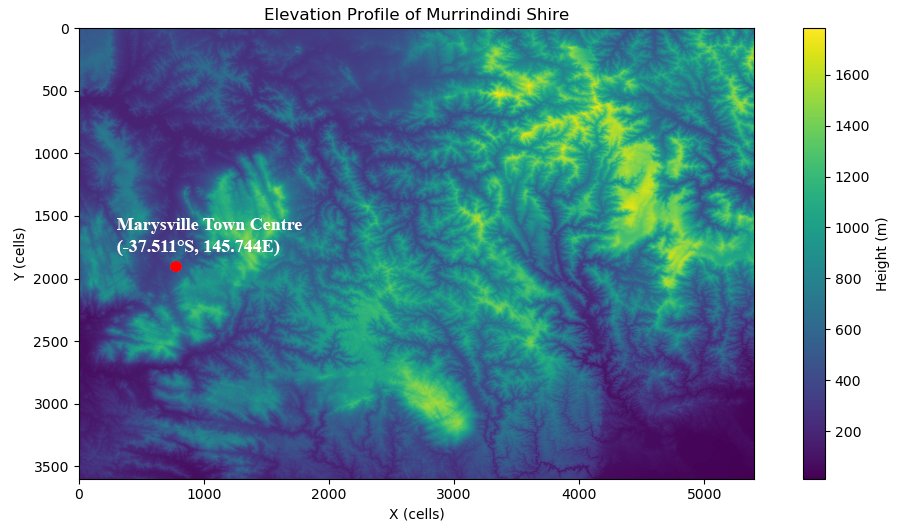
\includegraphics[width=0.83\textwidth]{Figures/elevation.png}\caption{Elevation data for Murrindindi Shire, $(38.00 -37.00)$\degree S, $(145.50 - 147.00)$\degree E}\label{topography}
\end{figure}

The relief map in Figure \ref{topography} shows substantial elevation changes in the region, where altitude changes from a minimum of $13$ metres to a maximum of $1783$ metres in less than $50$ kilometers on the ground. Wildfire has a tendency to travel uphill faster than downhill, and we expect our model to simulate this effect in the regions where the local surface gradient is the most pronounced. The data for elevation is used to calculate the fire propagation coefficients as described in Section \ref{factors}.\newline
\indent For the vegetation data, we use a topographical map with forest coverage data, accessed through Geoscience Australia's Web Portal \cite{Geodata}. We binarize the landscape into two possible values: cells with forest cover are assigned a value of $0$ (fuel), and cells without forest are assigned a value of $1$ (non-flammable). The output is shown in Figure \ref{forestcover}.

\begin{figure}[h!]
\centering
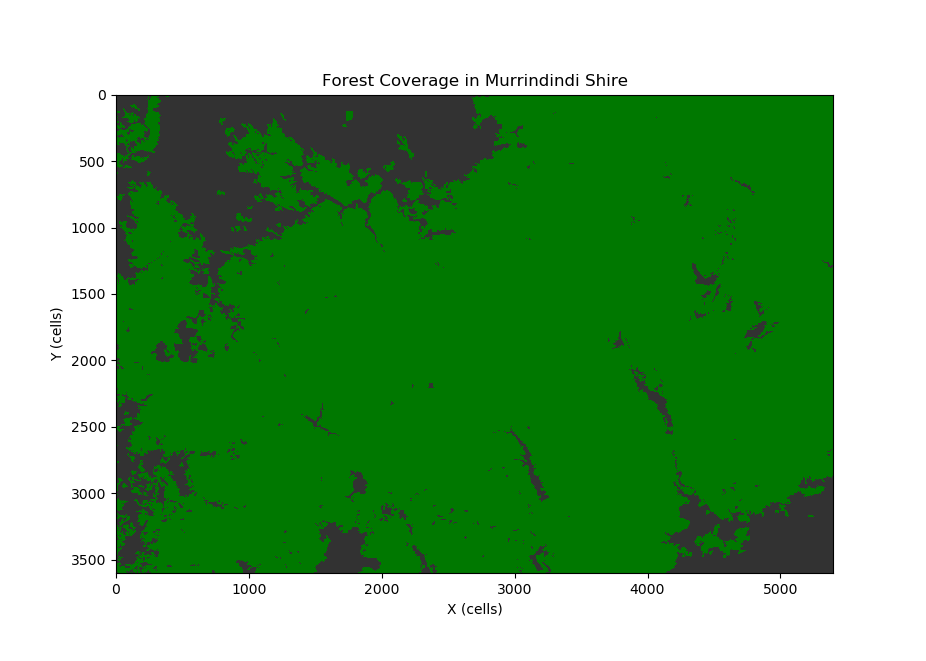
\includegraphics[width=0.9\textwidth]{Figures/ForestCover.png}\caption{Map of forest coverage in Murrindindi Shire. Woodland is represented by green and non-flammable terrain (including water) is shown in gray.}\label{forestcover}
\end{figure}

\noindent To analyse our model in the simulated real-world scenario of the Murrindindi fires, we perform a simulation of duration $N=500$ time steps, with different sets of environmental variables on each run. The cell arrays for elevation and vegetation were resized to dimensions $(540 \times 360)$ to maintain a feasible run time. The fire duration $\Delta t$ was configured to $2$ time steps, and the strength parameters $\alpha$ and $\beta$ and spotting parameters $E,M$ and $\sigma$ are varied across different runs. The results are shown in Figures \ref{fig:vegeOnly} to \ref{fig:allParams}, and we compare these to the real observations of the bushfires, shown in Figure \ref{fig:realData}.

\subsection{Fire Simulation Results}
\begin{figure}[H]
  \centering
  \begin{subfigure}[t]{0.47\textwidth}
    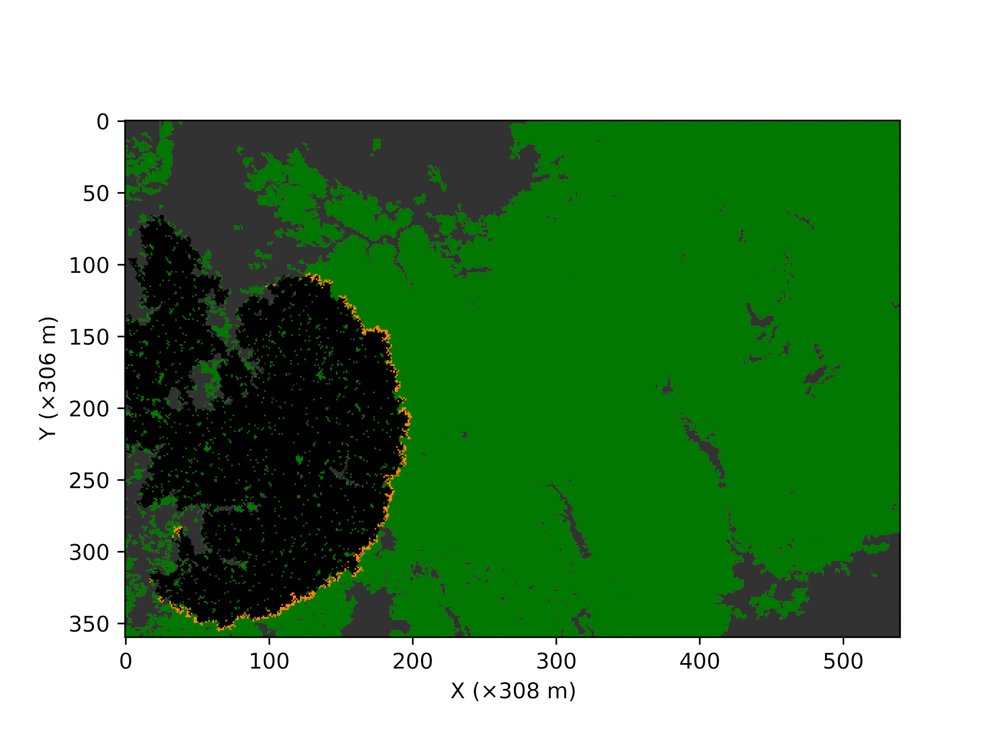
\includegraphics[width=0.95\textwidth]{Figures/LastFrame_01.jpg}
    \caption{Simulation run with vegetation data only, \,\, iterated for a duration of $500$ time steps}
    \label{fig:vegeOnly}
  \end{subfigure}
  %
  \begin{subfigure}[t]{0.47\textwidth}
    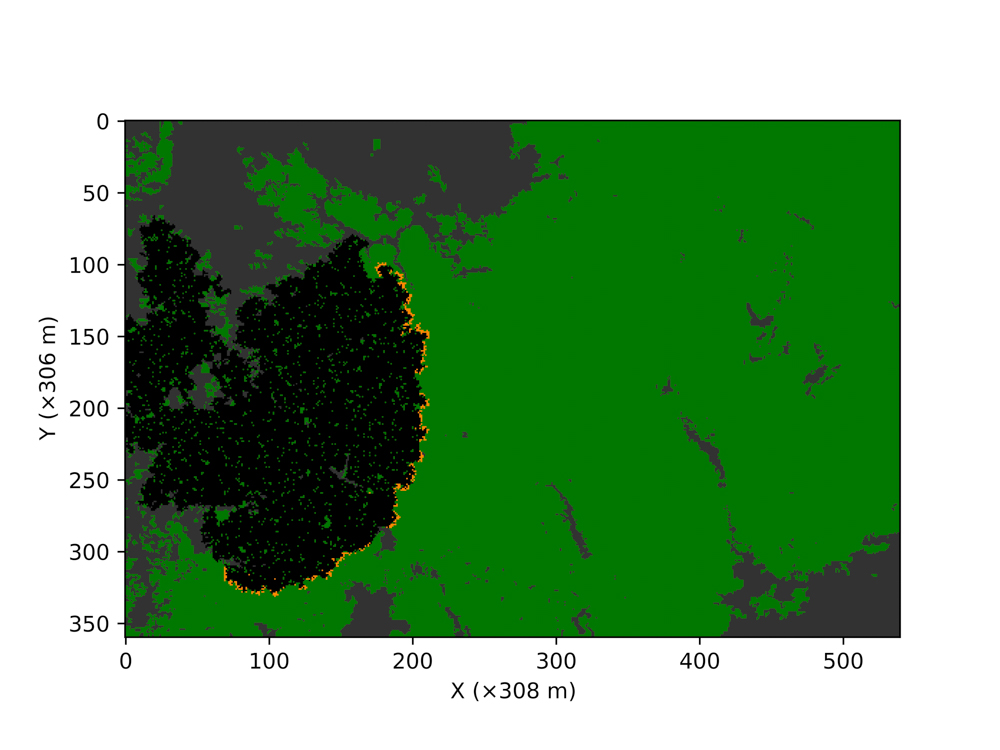
\includegraphics[width=0.95\textwidth]{Figures/LastFrame_02.jpg}
    \caption{Simulation with vegetation and elevation data, $\alpha=0.045, \beta = 0$, iterated $500$ time steps}
    \label{fig:vegePlusEle}
  \end{subfigure}
  %
  \begin{subfigure}[t]{0.47\textwidth}
    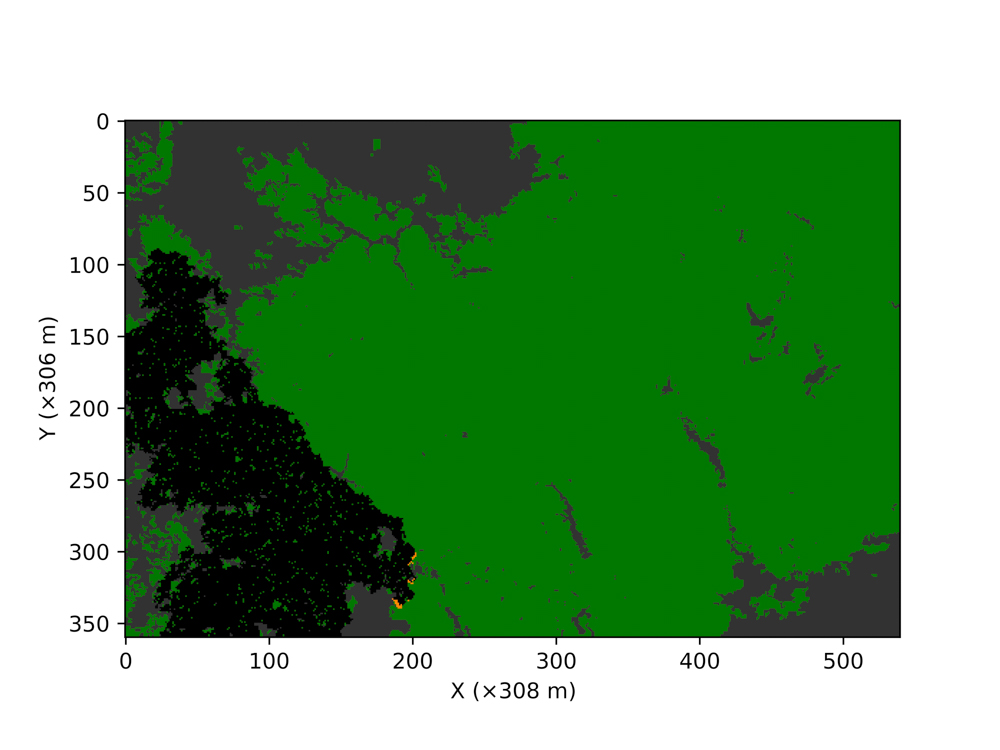
\includegraphics[width=0.95\textwidth]{Figures/LastFrame_03.jpg}
    \caption{Simulation with vegetation and wind data, $\alpha=0, \beta = 0.1$, iterated $500$ time steps}
    \label{fig:vegePlusWind}
  \end{subfigure}
  %
  \begin{subfigure}[t]{0.47\textwidth}
    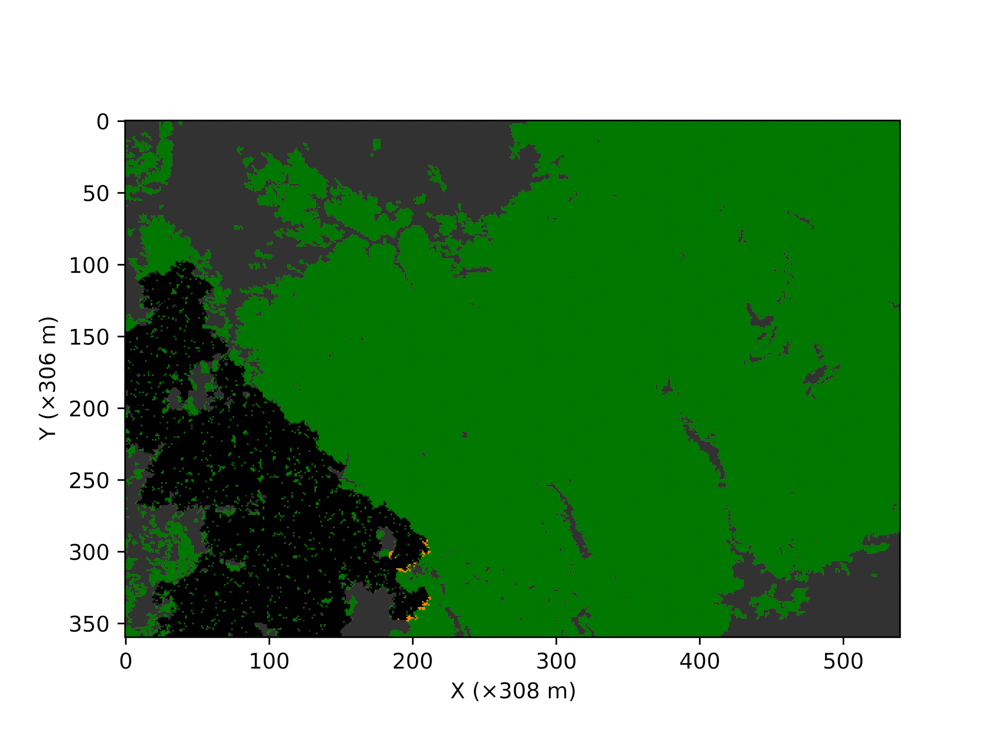
\includegraphics[width=0.95\textwidth]{Figures/LastFrame_04.jpg}
    \caption{Simulation with vegetation, elevation and wind data, $\alpha=0.045, \beta = 0.1$, $500$ time steps}
    \label{fig:vegePlusElePlusWind}
  \end{subfigure}
  %
  \begin{subfigure}[t]{0.47\textwidth}
    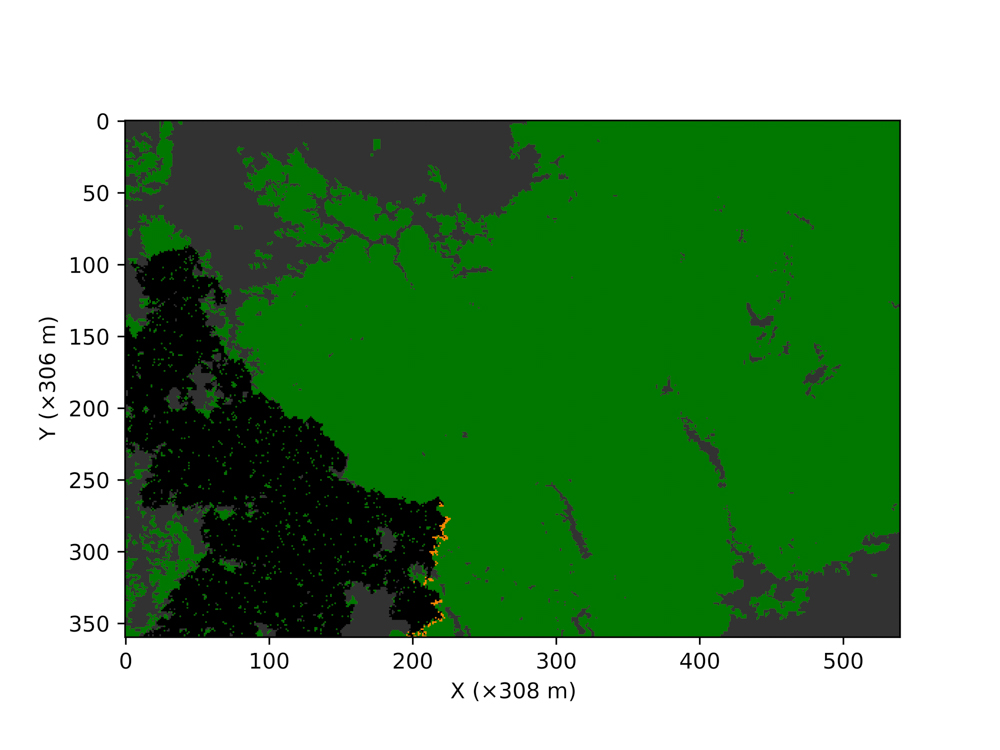
\includegraphics[width=0.95\textwidth]{Figures/LastFrame_05.jpg}
    \caption{Simulation with vegetation, wind and ember data, $\alpha=0, \beta = 0.1$, iterated $500$ time steps}
    \label{fig:almostAllParams}
   \end{subfigure}
   %
   \begin{subfigure}[t]{0.47\textwidth}
    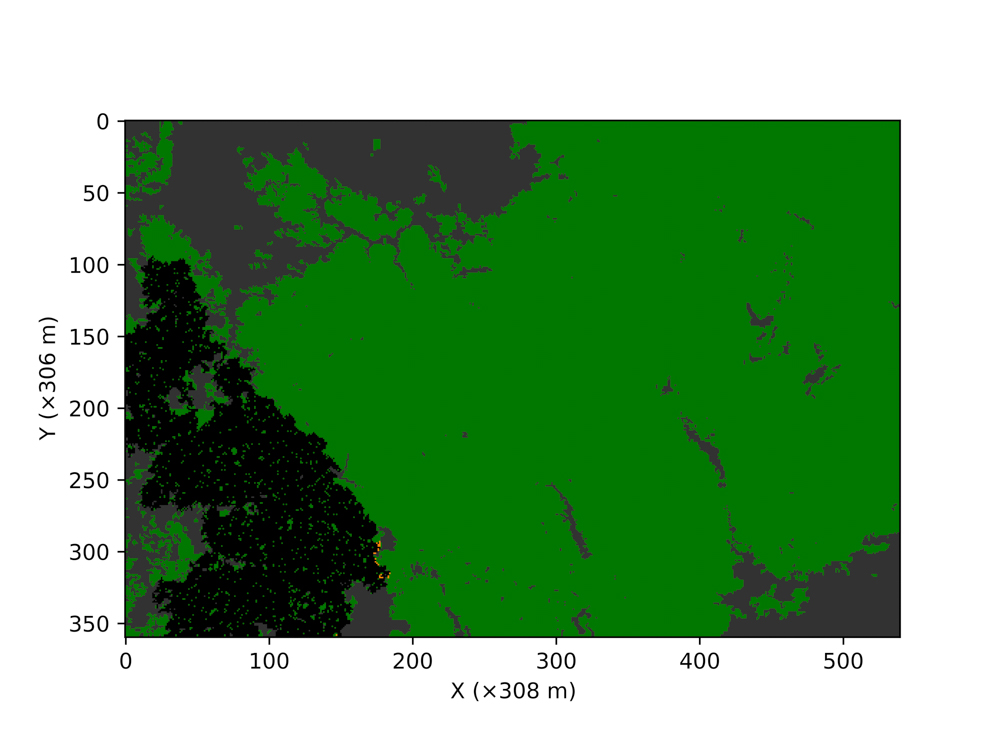
\includegraphics[width=0.95\textwidth]{Figures/LastFrame_06.jpg}
    \caption{Simulation with vegetation, elevation, wind and ember data, $\alpha=0.045, \beta = 0.1$, $500$ steps}
    \label{fig:allParams}
   \end{subfigure}
   \caption{End result of Murrindindi fire simulation after 500 time steps.  Colour code: \newline green = fuel cells, orange = fire cells, black = burnt cells, grey = non-fuel cells.}
\end{figure}

\noindent In Figure \ref{fig:vegeOnly}, we observe that the fire front is uniform in the flammable area, and approximately symmetrical around its centre. This demonstrates that in the absence of other factors, fire will propagate evenly in all directions where fuel is present. In Figure \ref{fig:vegePlusEle}, the added elevation data breaks the symmetry of the fire front, and fires have preferential directions based on the surface gradient.\newline \indent
For the simulation using wind data, we configured the wind velocity to $52$ km/h South-South-Easterly, as measured at the local Coldstream Automatic Weather Station at 18:00 \cite{RoyalCommission}. The effect of wind is seen in Figure \ref{fig:vegePlusWind}, where the fire front propagates uniformly along the direction of the wind, with only minor deviations from the path. When the effects of elevation and wind are combined, we observe that wind largely dictates the direction of the fire, as seen in Figure \ref{fig:vegePlusElePlusWind}. Here, the resulting path of fire is almost identical to that traced out in Figure \ref{fig:vegePlusWind} where wind is the only additional factor. \newline \indent
To test the effect of spotting on the path of fire, we configured each burning cell to send out $E=10$ embers, which remain on fire for a duration of $t_f = 30$ seconds. A fuel cell was set to ignite on average by $M=50$ embers, with a standard deviation of $\sigma=10$. The result of a simulation incorporating wind and ember data is shown in Figure \ref{fig:almostAllParams}. We observe that the effect of spotting speeds up the rate of fire spread along the direction of the wind, visible at the bottom of the map where the fire front has advanced further South than it did in the simulation with wind data alone.\newline \indent
For the final test, we ran the simulation using all available parameters: elevation, wind and spotting. The result after $500$ time steps is displayed in Figure \ref{fig:allParams}. We remark that the end result is comparable to previous results with wind data, with a small difference in the lower section of the map where the change in elevation at the bottom of the map inhibited the fire from propagating to certain downhill areas.

\subsection{Comparison to Real Events}
To assess the accuracy of the model, we compare its results to the actual events of the Murrindindi fires, as captured by satellite images. In totality, the Murrindindi fire burnt an area of $43,154$ hectares over the course of $27$ days. We analyse the differences between our model and real-world events by calculating the total surface area burnt in the fire simulation, and compare these values to the actual area burnt by the real fires. Due to a long run time of $\sim 7$ hours for each simulation, the data obtained is a direct non-averaged output generated in a single instance. The results are presented in Table \ref{Tab:areaburnt}. \newline
\indent We observe that our model significantly overestimates in the amount of area burnt when compared to the physical events, and our results differ from the target of $43,154$ hectares by up to two orders of magnitude (Figure \ref{fig:vegeOnly}). Based on the area burnt, the most accurate versions of the model include the effects of wind (Figures \ref{fig:vegePlusWind} - \ref{fig:allParams}). This suggests that wind is a primary factor in determining the accuracy of a wildfire simulation.

\newpage

\begin{table}[h!]
    \centering
    \begin{tabular}{|c|c|}
    \hline
     \textbf{Figure} & \textbf{Area burnt} (ha)\\ \hline
     \ref{fig:vegeOnly} & $1,137,690$ \\ \hline
     \ref{fig:vegePlusEle} & $1,039,539$ \\ \hline
     \ref{fig:vegePlusWind} & $254,428$\\ \hline
     \ref{fig:vegePlusElePlusWind} & $389,184$\\ \hline
     \ref{fig:almostAllParams} & $370,444$\\ \hline
     \ref{fig:allParams} & $425,608$\\ \hline
     \ref{fig:realData} (target) & $\mathbf{43,154}$\\ \hline
    \end{tabular}
    \caption{Total surface area burnt in wildfires as $t\xrightarrow{}\infty$}\label{Tab:areaburnt}
\end{table}

\noindent In the case of Figures \ref{fig:vegeOnly} and \ref{fig:vegePlusEle}, the surface area burnt in the simulation is approximately $90\%$ of the total area of flammable material. This is in contrast to the real events, where the fires remained localised in the Marysville area and were confined  within a $\sim 25$km radius of the town centre. An infrared image of Marysville and its surroundings on February 16\textsuperscript{th}, 2009 is provided for reference in Figure \ref{fig:realData}:

\begin{figure}[h!]
    \centering
    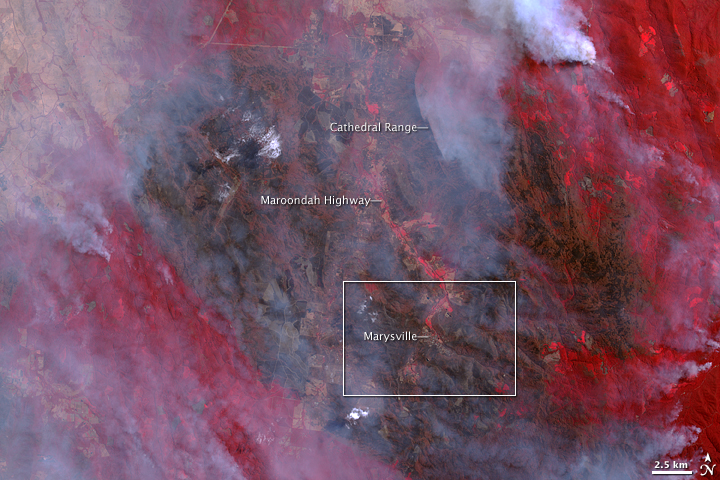
\includegraphics[width=0.9\textwidth]{Figures/realFire.jpg}
    \caption{Murrindindi fires (infrared image), 16/02/2009, NASA Earth Observatory \cite{NASA}}
    \label{fig:realData}
\end{figure}

\noindent We note that the above results vary substantially for different values of the strength parameters $\alpha$ and $\beta$. Previous work has determined that a value of less than $0.1$ for both $\alpha$ and $\beta$ shows the most accurate behaviour \cite{Aleksandridis_2008}, however the exact values need be determined via non-linear fitting methods such as Nelder-Mead optimization \cite{Denham_2018}. As determined in Section \ref{modellimits}, there are parameter-specific limits at which the fire behaviour becomes non-physical. To avoid this we selected the values $\alpha = 0.045$ and $\beta = 0.1$ for elevation and wind respectively. \newline
\noindent For the parameters related to embers, our method is novel to the literature. As such, there was no previous analysis on the ideal number of embers emitted by fire, and we determined the values $E=10, M=50$, $t_f = 30s$ and $\sigma=10$ based on trial and error.\newline \indent
We postulate that the main reason behind the discrepancy between our model and the real-world events is the static nature of the environmental conditions in our model. Firstly, the wind speed and direction is a fixed variable in our model, whereas in the real world there were major changes in wind direction occurring on February 7\textsuperscript{th}. Secondly, the real bushfires burnt out as a result of a change in weather conditions and continued human efforts, whereas our model lacks these stabilising factors. Thirdly, our cellular automaton is defined using a binary criterion where a cell is either flammable or not, so it does not fully represent different types of possible fuel. In a real environment, a bushfire has a different ignition probability than a canopy or a grass fire, and the fire duration varies across different vegetation types. \newline\indent
We theorise that the lack of moderating factors in our model causes the simulated fires to spread out until most of the fuel source is burnt, especially in the models without wind effects. An example of this is shown in Figure \ref{fig:endFrame}, where we show the state of a Murrindindi simulation with $\Delta t=2$ after $1000$ time steps using vegetation data.

\begin{figure}[h!]
    \centering
    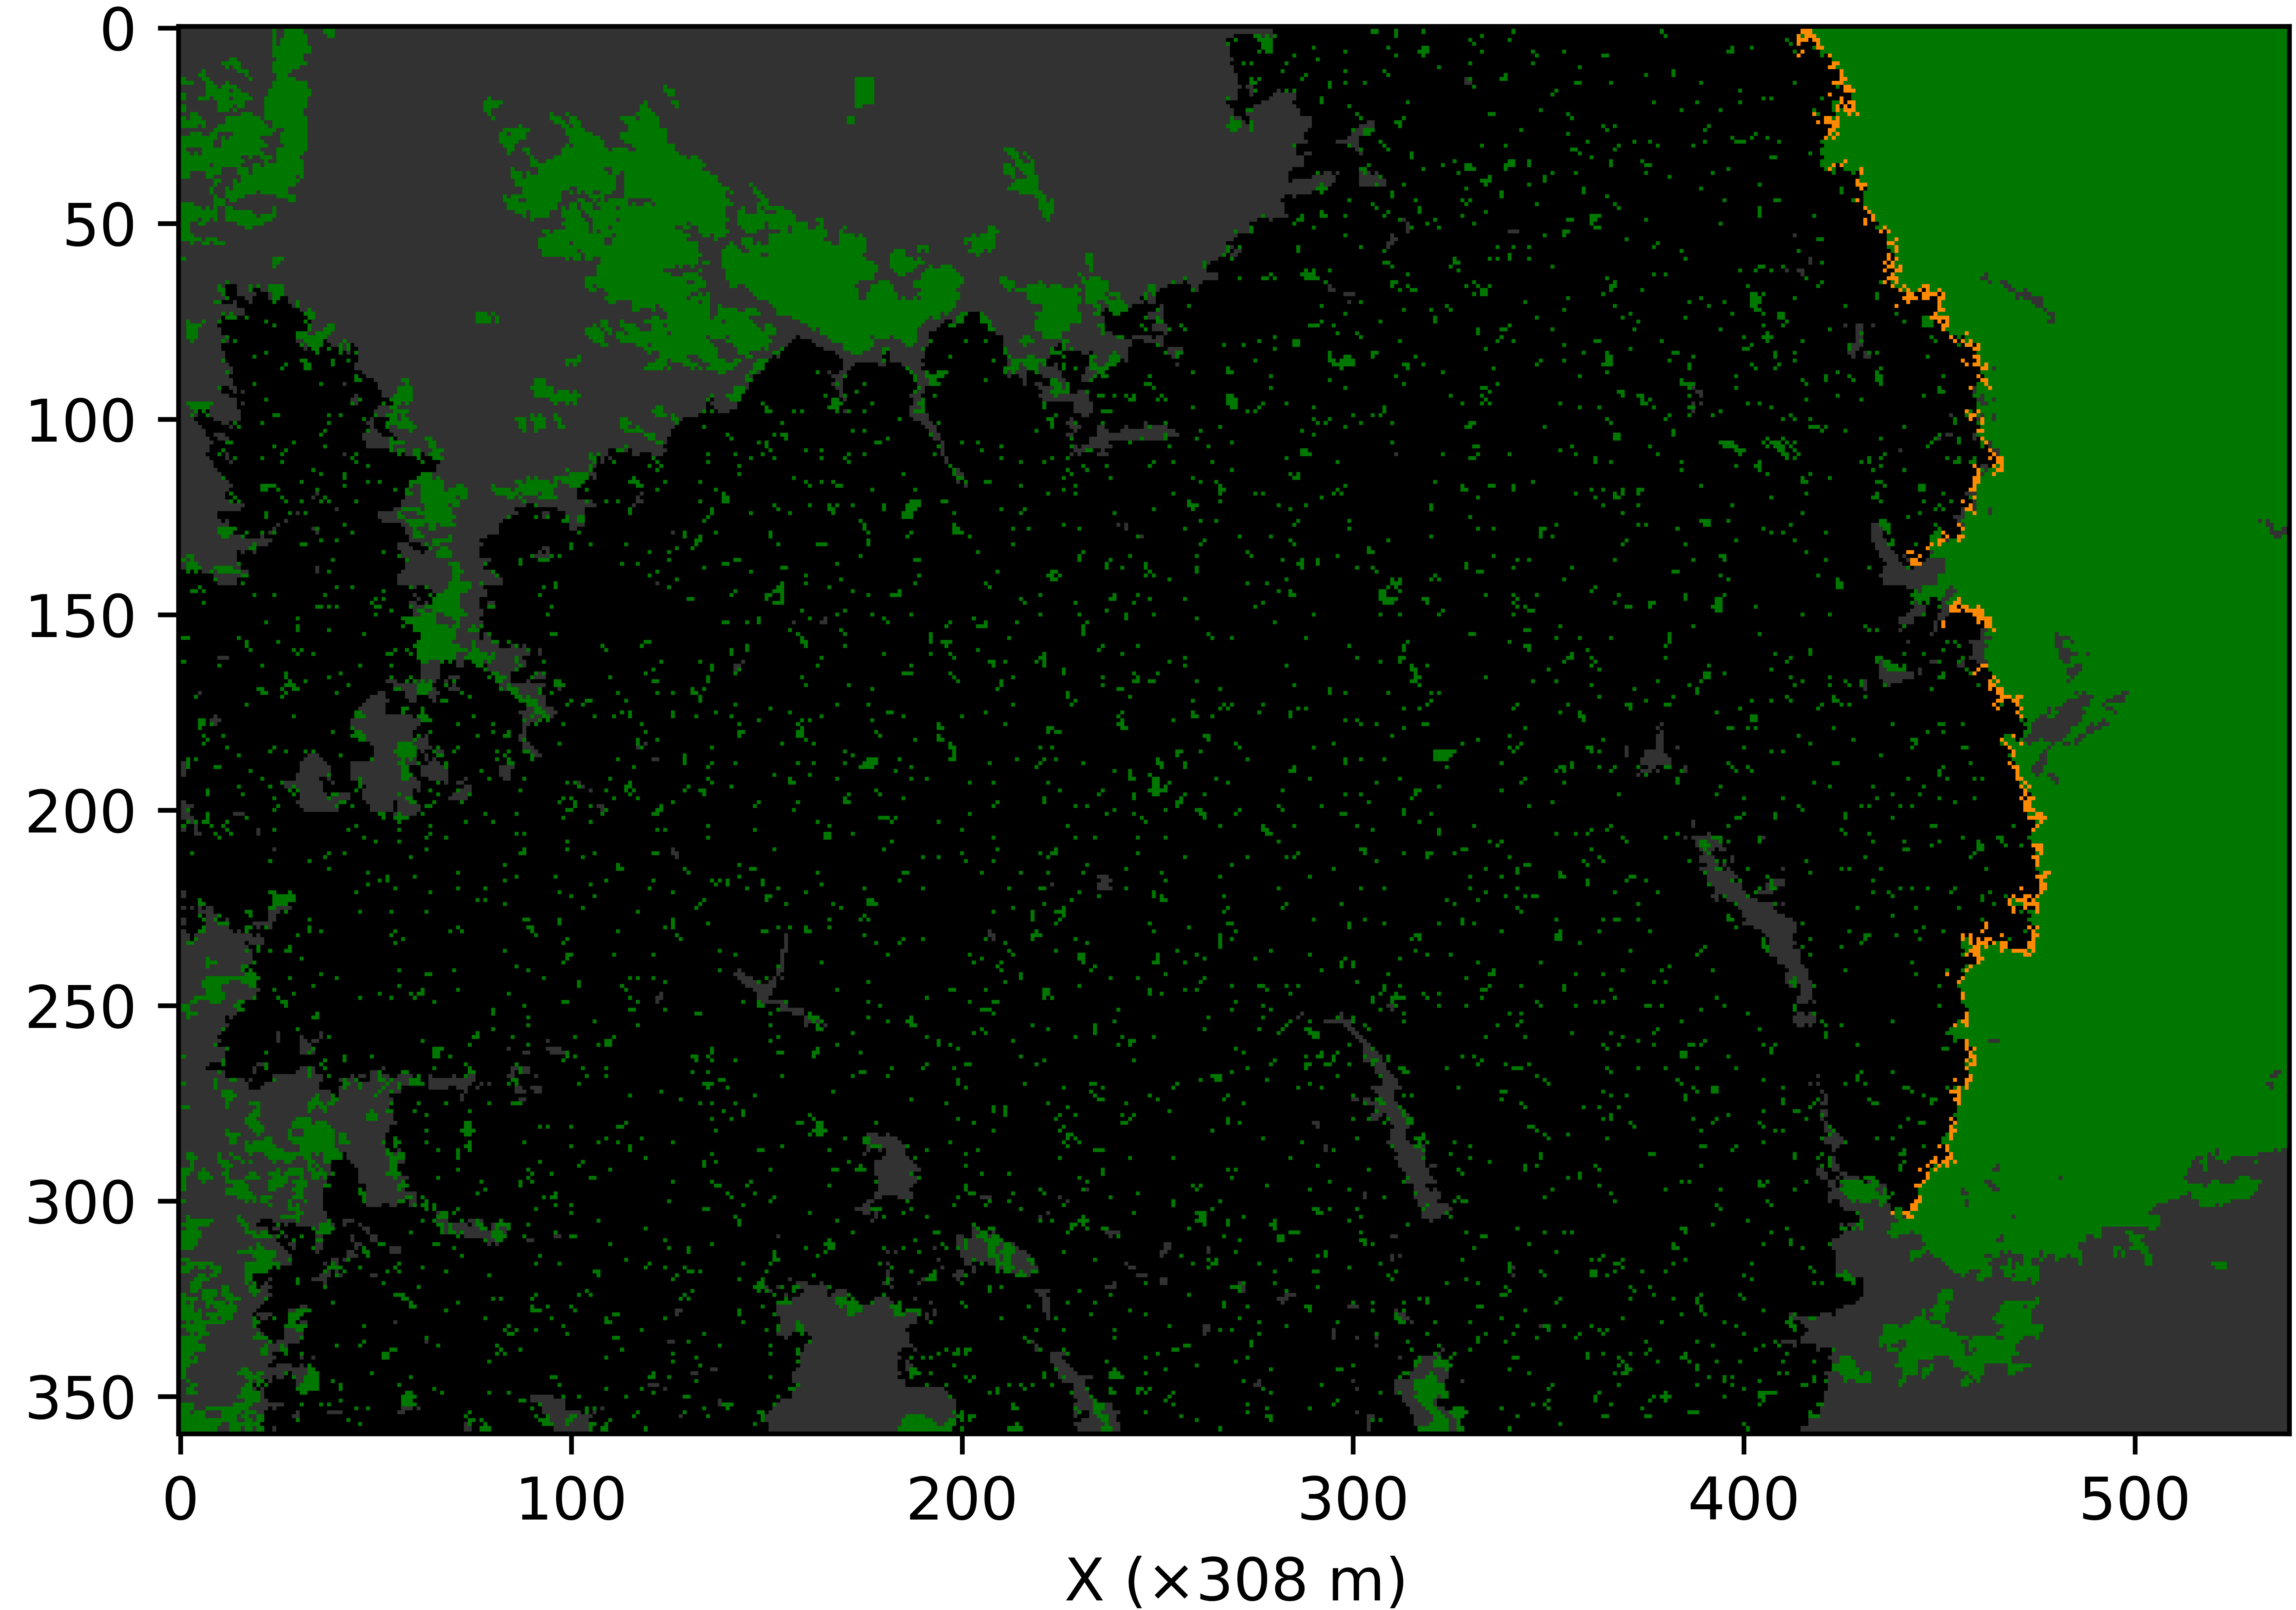
\includegraphics[width=0.5\textwidth]{Figures/LastFrame.png}
    \caption{End result of fire simulation, duration 1000 time steps.}
    \label{fig:endFrame}
\end{figure}

\indent We observe that in the absence of wind, the fire spreads unconstrained across the whole landscape, burning over $90\%$ of the fuel source. This is an unrealistic result, as real wildfires tend to extinguish over time due to changes in weather conditions. To overcome this limitation in our current simulation, a more accurate model must reflect possible environmental changes in the net fuel ignition probability. Further work is also required to determine the control parameters $\alpha,\beta,E,M,t_f$ and $\sigma$ to balance the effect of elevation, wind and spotting. To this end, we suggest improvements to the model in Section \ref{furtherwork}.

pot\newpage
\section{Conclusions}\label{conclusions}

\subsection{Accuracy of the Model}

We present a novel cellular automaton approach for modelling wildfires, using an adaptation of previous work by A. Aleksandridis \textit{et al.} in 2008 \cite{Aleksandridis_2008} and A. Quartieri \textit{et al.} in 2010 \cite{Quartieri_2010}. The environmental parameters of elevation, wind and spotting are added to this model to recreate fire wildfire behaviour as accurately as possible. We analyse how the introduction of each of these parameters affects different aspects of fire behaviour, including the shape of the fire front and the rate of spread. Our model allows us to quantify these effects using a set of equations that describe the probability of ignition of an arbitrary cell, presented in Equation \ref{p2}. Despite an uncertainty of $\sim 15-20\%$ in the fuel ignition probability, our model shows good predictive potential. \newline \indent We apply our model to simulate the events of the 2009 Australian bushfires, with mixed results. Our cellular automaton model exhibits wildfire-like behaviour in the simulated physical environment of Murrindindi, with specific limitations. The fires follow the direction of the wind and travel uphill faster than downhill, and the simulated fires travel through the town of Marysville as expected. We determine that the most important physical variables in the simulation are the speed and direction of wind, when measured by the accuracy in predicting the total area burnt. These findings are supported by existing literature \cite{Xuehua_2016, Freire_2019}, giving us confidence in the validity of our approach. Although the basic behaviour of wildfire is recreated, the model requires fine-tuning before it can be accurately applied to real geographical systems, as it substantially overestimates the surface area burnt by the wildfires. To improve the simulation we propose additional factors as described in Section \ref{furtherwork}.

\subsection{Proposals for Future Work}\label{furtherwork}

To generate reliable real-world predictions from our model, we propose that the direction of the wind be implemented as a time-dependent vector map. This will allow the fire to change direction along possible wind changes, which should significantly improve the simulation accuracy. We also suggest that the values of the strength parameters $\alpha$ and $\beta$ be determined through a Monte-Carlo simulation, so that the results of the simulation match real-world events as accurately as possible. To do this, we suggest modifying the parameter optimisation procedure developed by M. Denham and K. Laneri for fire simulations in 2018 \cite{Denham_2018}. Finally, we propose that the model be tested on a variety of past fire events to verify its validity and see if the constants $\Delta t,\alpha,\beta,E,M,t_f$ and $\sigma$ are universal across different landscapes. \newline \indent A brief investigation into the wildfire effects on the local populations in Marysville was conducted alongside the main project. A summary of our methodology and initial findings is found in Appendix \ref{population_appendix}. Combining cellular automata models for both fire simulation and population movement allows an insight into how different parameters influence the eventual number of casualties in the fires. Ultimately, such a model could be used to predict high risk areas or be used to adjust bushfire survival advice before the events happen.

%---------Acknowledgements-----------------------

%---------Appendix-------------------------------

\newpage
\appendix

\section{Code Overview}\label{code}

\begin{figure}[h!]\label{flowchartcode}
\centering
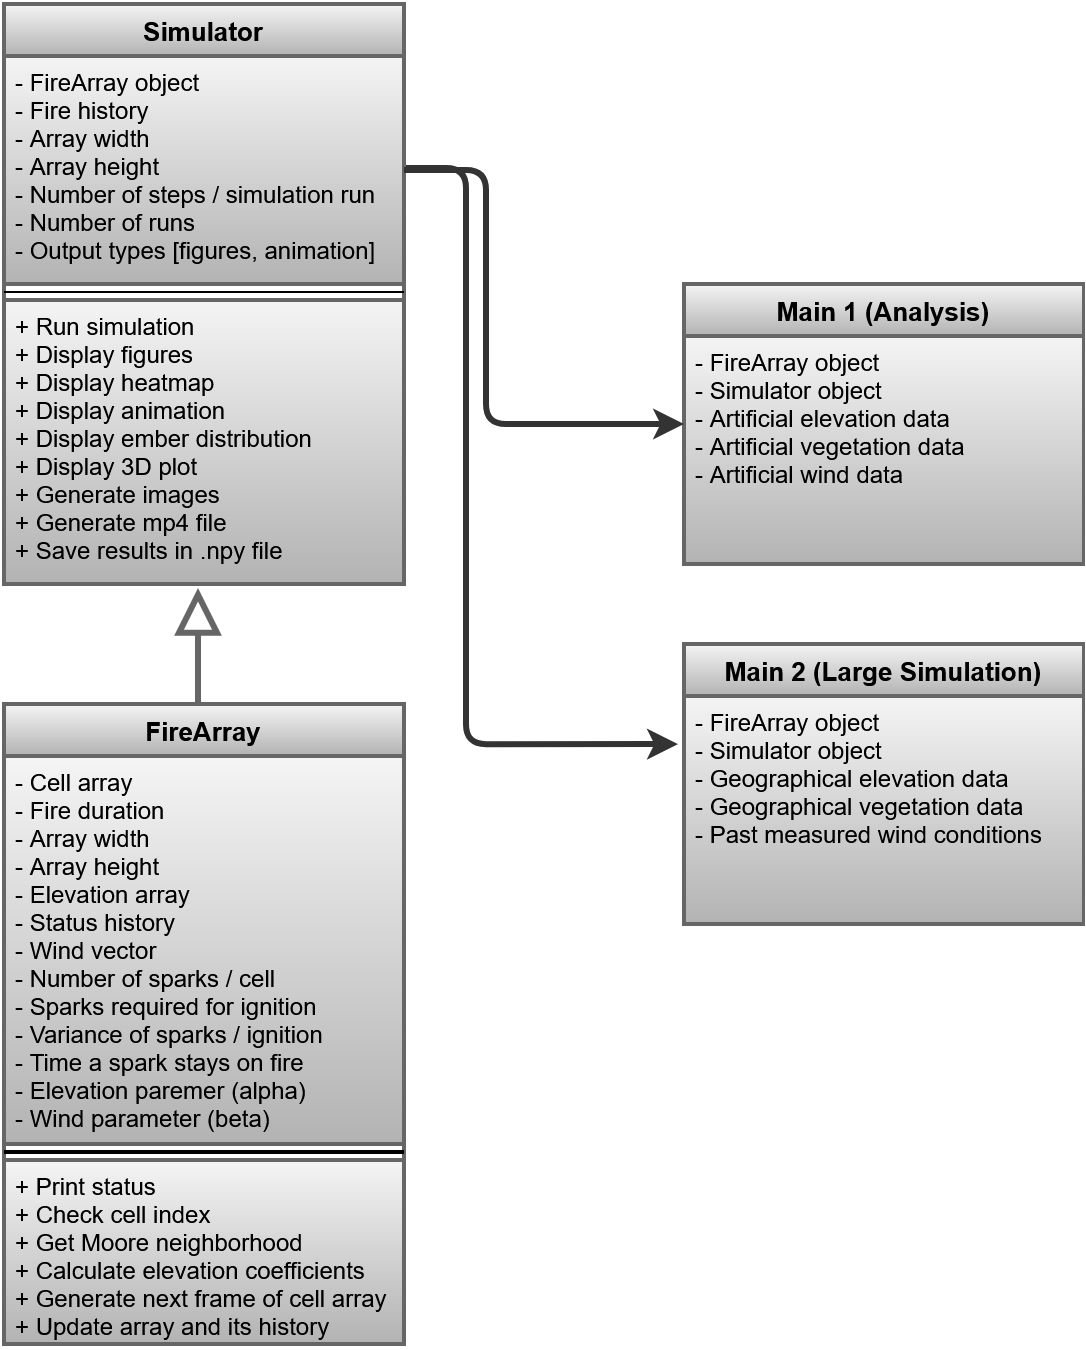
\includegraphics[width=0.8\textwidth]{Figures/FireArray.png}\caption{Class diagram for simulation code. The program is run using instances of FireArray objects, which represent the cellular automaton. The simulation and its outputs are handled by the class Simulator, which is controlled by the user via programs Main 1 and Main 2.}
\end{figure}

\section{Population Study Detail}\label{population_appendix}

Our primary motivation in understanding population behaviour is to identify the key attributes for the preservation of life. Modelling human behaviour is notoriously difficult as no two people will have the exact same reaction in a given scenario. Hence to build a relatively accurate model, one must make a series of assumptions. The fight or flight instinct was used heavily as a basis for decision making. Proportions of fight or flight populations were assimilated from 4.2.5 in J. Handmer \textit{et al.} \cite{J_Handmer}, note that this data was normalised as some populants conducted more than one key action.

\begin{figure}[h!]
    \centering
    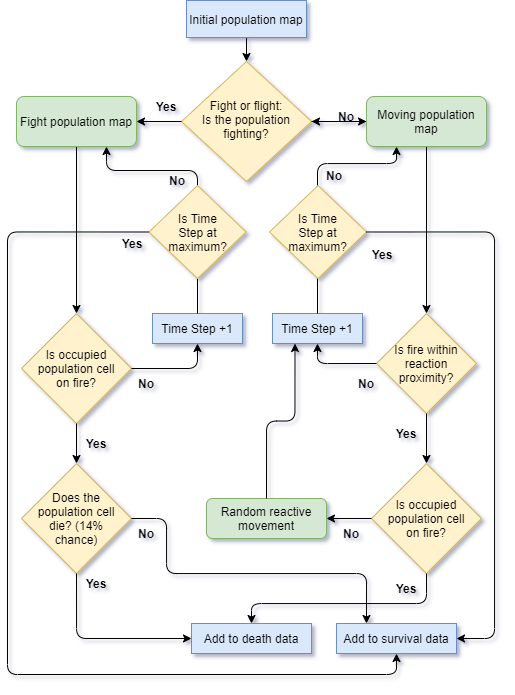
\includegraphics[width=0.65\textwidth]{Figures/population_flow.png}
    \caption{A flow chart depicting the general code decision making process for the population model. This code was able to take an initial population density map and conduct iterations up to a maximum time step. All of the deaths in the simulation were stored with the time, location and action at the time of death. This data could then be used for analysis.}
    \label{population_flow}
\end{figure}

The 'fighting' and 'flighting' populations were split and run simultaneously with the fire simulation. Fighting populants were given a 14\% probability of death if they occupied the same cell as an active fire, this mark was also determined from 4.2.5 in J. Handmer \textit{et. al}. Flighting or 'moving' populations were set up to detect fire in 4 separate cardinal regions (SE,NE,SW,NW) within a given proximity. Based on which regions detected a fire, a random reactive movement within a Moore neighbourhood resulted so that the populant would move in a general direction away from the fire(s). A summary of the coding process is offered in figure \ref{population_flow}.

\begin{figure}[h!]
    \centering
    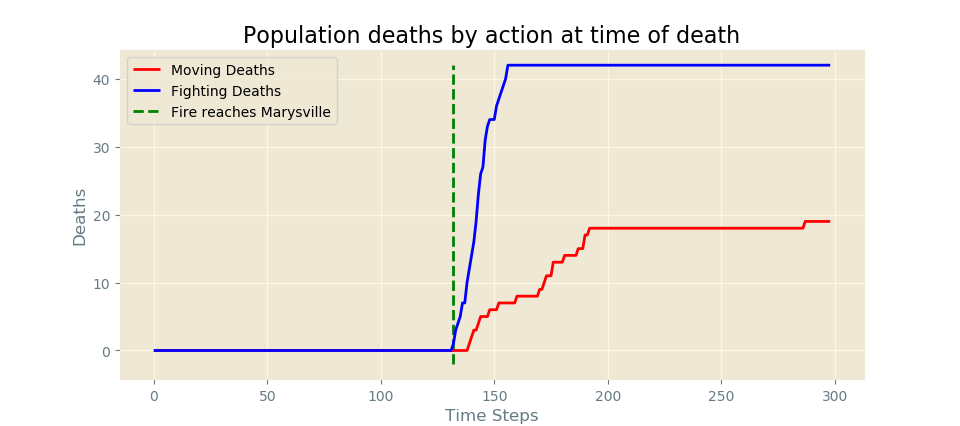
\includegraphics[width=1.0\textwidth]{Figures/fight_vs_flight_deaths.png}
    \caption{A comparison of deaths as a result of populations fighting the fire or moving away from the fire. An initial population of 500 was used with focused density at the location of Marysville. The fire simulation used had parameters of wind and elevation included.}
    \label{forf}
\end{figure}
Upon scrutiny of the data obtained, it was clear that the fighting group were at a higher risk of fatality than the moving group. This is displayed in figure \ref{forf} and is in adequate agreement with J. Handmer \textit{et. al} data. Given this understanding we can begin to present a motive to not fight a fire.
\begin{figure}[h!]
    \centering
    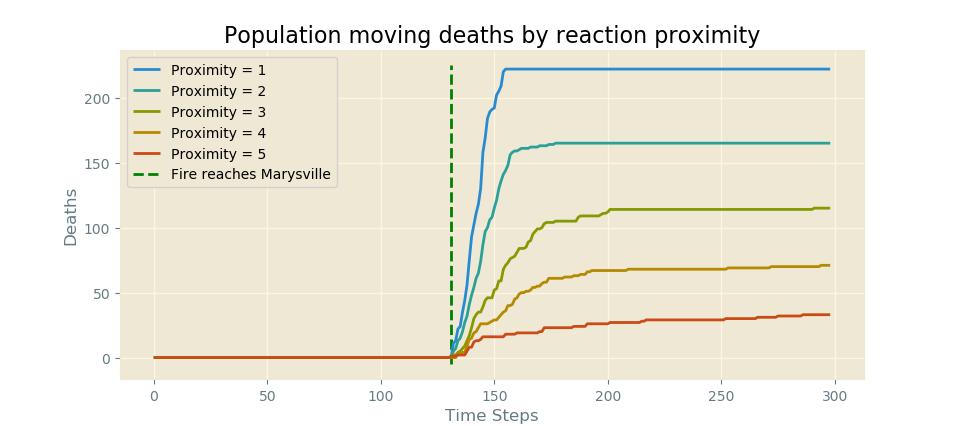
\includegraphics[width=\textwidth]{Figures/proximity_deaths.png}
    \caption{A comparison of moving deaths as a result of varying cellular reaction proximities. The same initial conditions were used as in figure \ref{forf}. The cardinal reaction regions were set square to reduce computational effort. Maximum deaths (\textit{i.e.} all of the moving population) occurred at a proximity of 1.}
    \label{proximity_deaths}
\end{figure}
A further interesting comparison is the effect of reaction proximity on death rate. Figure \ref{proximity_deaths} supplies another clear observation that the larger the reaction proximity (\textit{i.e.} the distance at which a fire needs to be in order to cause a populant to move), the higher the survival rate. This highlights the importance of making sure that populants evacuate as soon as the risk is near. This is a key finding of the Victoria Royal Bushfire Commission - 'leaving early is [still] the safest option'. \newpage \noindent In conclusion there is a lot to be learned from studying cellular automata fire-population models with the potential promise of offering life saving advice and techniques. As a direct result of the 2009 Australian bushfires, the Victorian Royal Bushfires Commission reviewed their 'stay or go' policy \cite{RoyalCommission} as it was found that it was not effective for the scale of fire experienced on Black Saturday. Modern methods now include SMS\footnote{SMS (also know as text messaging) is a mobile phone service that conveys specific messages between devices.} warnings of nearby bushfires in order to maximise survivability. Unfortunately these changes came too late for the 173 people who died in the 2009 Australian Bushfires, demonstrating the importance of such modelling.

\clearpage

\section{Project Management}\label{management}
This section contains the project plan, a Gantt chart for the projects planned progression and a complete record of all meeting agendas and minutes. The Project Plan was written at the beginning of the project to determine general objectives for the group. The agendas and minutes for meetings were recorded throughout the project.
\subsection{Project Plan}

\small

\hspace{\parindent}\textbf{Timetable}: Lent Term W11-20 \hspace{1cm} \textbf{Members}: Joonas, Joe, Antony, Alex

\textbf{Project Objectives}
\begin{itemize}
    \item Physical Background:\begin{itemize}
        \item Simulate the bushfires taking place in South-eastern Australia over the events of Black Saturday using cellular automata models.
        \item Display the evolution of the fires in the region of Murrindindi, Victoria, focussing on the town of Marysville
        \item Compare the simulation results with real data over how the fires evolved and their impact on the area and its inhabitants 
        \item Utilise real-world geographical and weather data as basis for the simulation
    \end{itemize}
    \item The Code: \begin{itemize}
        \item Writing an object-oriented program for CA simulation, using NumPy arrays and MATLAB for data acquisition
        \item Output: data about fire spread, area burnt, casualties and survivors, probability distributions of damage over critical areas
    \end{itemize}
    \item Physics Questions: \begin{itemize}
        \item Investigating how well the CA approach works as a physical model, compared to analytical alternatives such as diffusion models.
        \item Determine parameters which impact the fire damages the most
        \item Quantify the dependency of the model on physical parameters such as:
        \begin{itemize}
            \item Fire type (grass fire, bushfire, canopy fire)
            \item Fuel load (bark, leaf litter, grass etc.) \& fuel moisture
            \item Weather: wind speed \& direction, ambient temperature, relative humidity
            \item Geographical: slope angle, terrain type, water presence
            \item Barriers (water, concrete, human infrastructure)
        \end{itemize}
    \end{itemize}
    \item Resources:
    \begin{itemize}
        \item \url{https://www.ga.gov.au/scientific-topics}
        \item \url{https://en.wikipedia.org/wiki/Black_Saturday_bushfires}
        \item \url{https://en.wikipedia.org/wiki/Kinglake,_Victoria}
        \item \url{https://en.wikipedia.org/wiki/Marysville,_Victoria}
        \item \url{https://en.wikipedia.org/wiki/Shire_of_Murrindindi}
    \end{itemize}
\end{itemize}

\begin{figure}[H]\label{ganttchart}
\centering
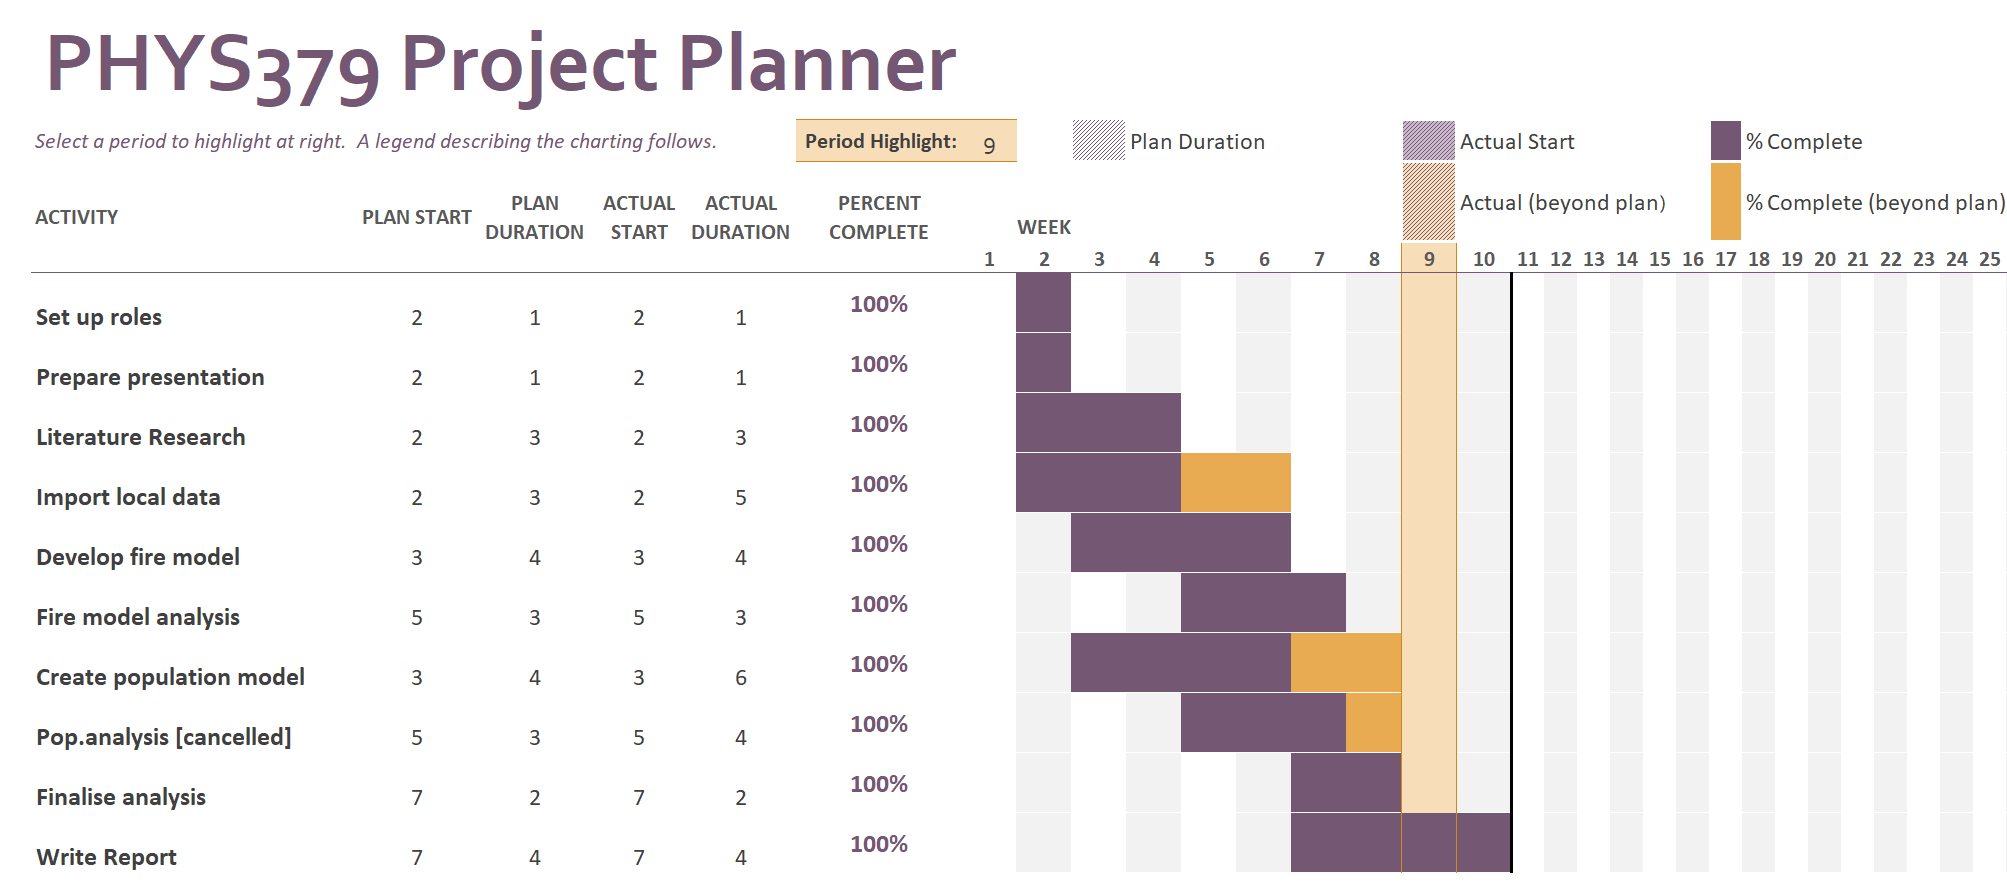
\includegraphics[width=\textwidth]{Figures/gantt_chart.png}\caption{Gantt Chart for group project, generated on 12/03/2020}
\end{figure}

\subsection{Meetings}

\subsubsection*{Week 2 Agenda \& Minutes}

\textbf{Meeting 1}

\noindent Location: Physics Building\newline
Date: 22/01/2020\newline
Time: 10:00\newline
Attendees: Joonas, Joe, Antony\newline
Apologies: Alex (TBC) 

\noindent\textbf{Agenda:}

\begin{itemize}
    \item  Assigning Roles - Set up and officiate roles for all group members: Coordinator = Joonas, Secretary = Joe.
	\item Splitting Work - Delegating each member for a specific task for next week: literature research, coding, data acquisition: split the project in 2 directions Joonas: maps, Joe: fire research, Antony: populations
	\item Project Plan - Signing and agreeing on the project plan, reading it together and making any changes
	\item Finalize Gantt chart - Set up milestones in the project and determine the general objectives 
	\item Discuss challenges - Discuss members’ coding abilities: determine easy/doable/hard tasks and assign them
	\item Common OneDrive - Set up a shared OneDrive folder for all common files: make sure all have access
	\item Additional info: Alex has not yet responded, waiting for reply
	\item Next Meeting: 28/01/2020, 10am @Physics
\end{itemize}
\clearpage
\noindent \textbf{Minutes:}

\noindent Joonas and Joe were appointed as chair and secretary respectively. The possibility of having a team name was discussed however no name was decided upon. The constitution was agreed upon and signed by Joonas, Joe and Antony. Ideas relating to the Australia Bushfire model were discussed. These ideas included: Modelling how the fire spreads throughout Australia; modelling how the population of trees and plant life were affected as the fire spread; modelling how the populations of both wild animals and humans were affected as the fire spread. Tasks were delegated for each attendee to attempt before the next meeting:  

\begin{itemize}
    \item Joonas - Creating a map of Australia of a cellular automata grid using MATLAB. 
    \item Joe – Research into how fire can be modelled using Cellular Automata. 
    \item Antony - Research into how movement of populations can be modelled using CA. 
\end{itemize}

\noindent \textbf{Meeting 2}\\
Location: In-Class, Man. LT 06\\
\noindent The project aim was discussed for the first time as a whole group. The unlikeliness of being able to create a cellular automata model containing the whole map of Australia was discussed. Possible alternative models were considered. Possible data that could be extracted from the model was also considered.  Tasks for the next meeting were updated: 

\begin{itemize}
    \item Joonas – Using maps of Australia to attempt to create a CA grid containing Australia 
    \item Joe – Finding literature to understand how fires spread and the effect of wind on their spread
    \item Alex – Creating initial code that can model fire 
    \item Antony – Finding literature to understand the movement of populations due to a large scale fire as well as fire prevention techniques
\end{itemize}

\subsubsection*{Week 3 Agenda \& Minutes}

\noindent \textbf{Meeting 3}\\
Location: Physics Building\newline
Date: 28/01/2020\newline
Time: 10:00\newline
Attendees: Joonas, Joe, Alex, Antony

\noindent \textbf{Agenda:}

\begin{itemize}
    \item Progress - Each member discussing their progress with the tasks given in the last meeting. Joonas: maps, Joe: research, Anthony: populations, Alex: N/A 
	\item Code - Group members to show progress with designing code for the project: split the task of coding into packages (ex. Fire, forest, wind, people…) 
	\item Gantt Chart - Update Gantt chart 
	\item Presentation Preparation - Designing a presentation in preparation for Thursday. Designating a particular topic to each member to rehearse for the presentation. 
	\item Future Work - Designate new tasks and goals to each member to attempt before next meeting. 
	\item OneDrive - Uploading any useful literature found by group members: Joonas to set up a folder on OneDrive 
	\item Next Meeting: Thursday 30/01 11:00
\end{itemize}

\textbf{Minutes:}

Alex was added to the shared OneDrive. Current progress with assigned tasks was discussed:

\begin{itemize}
    \item Antony – Literature on movement of populations and fire prevention techniques discussed
    \item Joe – Basic fire simulations from other sources were shown and literature on other fire simulations was discussed
    \item Joonas – His code for 1D automata and ‘Conway’s game of life’ was discussed
    \item Alex – His coding for a fire simulation was discussed
\end{itemize}

Gantt chart was updated to show the current progress of the project. Tasks to attempt during the next week were delegated:

\begin{itemize}
    \item Joe – Find data that will help make the model as realistic as possible, for example foliage cover certain parts of Australia
    \item Antony – Continue research and find parameters relating to population and fire prevention that could be added to the code
    \item Alex – Continue attempting to code fire simulations
    \item Joonas – Continue coding and attempt a simulation of fire
\end{itemize}

A group PowerPoint was created in preparation for Thursday was created and sections of the powerpoint were given to each member of the group:

\begin{itemize}
    \item Joe – Introducing the project
    \item Alex – Discussing how we aim to code a fire simulation
    \item Antony – Discussing population movements and preventative measures 
    \item Joonas – The difficulties of coding and the Gannt chart
\end{itemize}

A folder was created on the OneDrive so that any useful literature can be uploaded there.

\subsubsection*{Week 4 Agenda \& Minutes}
\noindent \textbf{Meeting 4}\\
Location: Physics Building\newline
Date: 04/02/2020\newline
Time: 15:00\newline
Attendees: Joe, Joonas, Alex, Antony

\noindent \textbf{Agenda:}
\begin{itemize}
	\item Progress - Each member discussing their progress: Joonas: fire code, Joe: geographical data, Antony: parameters for population/prevention model, Alex: fire code  
	\item Simulation plan - Joonas to explain the class structure of the CA code, determine aspects for each member to contribute to (wind, populations, etc) 
	\item Research questions - Members to come up with a physics question to answer in their investigation (ex. CA model vs diffusion, chaotic behavior, quantifying how well the model fits with physical laws [Symbol] stuff for report) 
	\item Define Objectives - Fire Simulation: \begin{itemize}
		\item Choose specific area, resolution and time for comparison (ex. Snowy Valley, 10,000 x 10,000 as hard target, town of Mallacoota 500 x 500 as easy target) 
		\item Populations \& Prevention: Antony to lead on this
		
		\item Physical parameters: 
		\begin{itemize}
			\item Grassfires vs bushfires vs canopy fires 
			\item Fuel load (bark, leaf litter, grass etc.) \& fuel moisture 
			\item Weather: wind speed \& direction, ambient temperature, relative humidity 
			\item Geographical: slope angle, terrain type, water presence 
			
			Analytical methods: someone to study how CA compares to other methods of fire modelling, maybe analytically?
		\end{itemize}
	\end{itemize}
	\item Next Milestones - Each member to commit to a deliverable for next week 
	\item Next Meeting: Thursday 06/02 1:30
\end{itemize}

\noindent \textbf{Minutes:}

The current progress of each group member’s assigned tasks was discussed:

\begin{itemize}
    \item Joe – Geographical data found during research was shown and explained to the group. Links to this data was uploaded to the OneDrive. Journals containing rules for automata when modelling fire were shown and then uploaded to OneDrive. Some research into mathematical models of wildfire not using cellular automata were discussed.
    \item Joonas – Python code that will be used for the simulation was shown and the class structure within the code was explained. This code was then used to show a fire simulation. Complications such as speed of run time with the code were discussed. Joonas explained how the data found by Joe could be implemented into the code.
    \item Antony – Flow chart showing how a population would react in the event of a wildfire was explained and discussed. Population data (how many people would leave etc.)  found during research was discussed. Ideas of how to code the movement of populations were then discussed.
    \item Alex – Progress with coding of fire simulation was discussed. Papers containing information about modelling wind were discussed.
\end{itemize}

\noindent Tasks to attempt in the next week were delegated. Group members should think of a physics question to answer in their investigation which could be mentioned in the final group report. As well as this each member should attempt to find data on a specific location that our simulation could be used to model. Individual tasks for the next week were:

\begin{itemize}
    \item Joe – Create short report on the different types of analytical modelling approaches. Use MATLAB to get geographical data into useable format.
    \item Joonas – Rewriting the simulation code such that it can be ran in a shorter time. Use MATLAB to get geographical data into useable format.
    \item Antony – Using literature on population movements to create some code that models a population. Use MATLAB to get geographical data into useable format.
    \item Alex – Create a 2D wind automaton and find useable data on wind speeds etc. 
\end{itemize}
\clearpage

\subsubsection*{Week 5 Agenda \& Minutes}
\textbf{Meeting 5}\newline
Location: Physics Building\newline
Date: 11/02/2020\newline
Time: 15:00\newline
Attendees: Joonas, Joe, Antony, Alex

\noindent\textbf{Agenda:}
\begin{itemize}
    \item Progress - Each member discussing their progress. Joonas: code \& geographical data, Joe: research on analytical approaches, Alex: wind model, Antony: code on population movement
    \item Simulation plan @Joonas - Confirm final parameters for fire model, to be programmed. Joonas: topography is doable within a week; fire hopping will take another (and will significantly affect runtime).
    Data acquisition: need a specific physical area to investigate. TBC during meeting, so that everyone can investigate the topic.
    \item Geographical Data @Joonas - Obtaining readable input data for simulation is crucial. Detailed elevation data is required, as well as data on flammable / non-flammable terrain. This will require information on vegetation cover, where a fixed threshold / criterion is needed to determine how flammable a cell is.
    \item Population Model @Antony - Status update: What is a realistic objective for this? What is the status of the code?
    \item Wind Model @Alex - Status update: is wind data possible to incorporate to the simulation within the timeframe?
    \item Analytical Methods @Joe - Report on the subject?
    \item Next milestones - Each member to commit to a deliverable for next week
    \item Next Meeting: Thursday 13:00
\end{itemize}
\textbf{Minutes:}

Current progress with each group members designated tasks were discussed:
\begin{itemize}
    \item Joonas – The current progress of the main fire simulation code was explained and discussed. The code was shown to the rest of the group and Joonas explained how the code has been altered to run faster and be easier to use. Joonas then explained how the code handles fire when it reaches the end of the automata grid as well as the how the rules implemented in the code were the same as those used by Quartieri in 2014. Joonas explained how the vegetation data from ‘Geoscience Australia’ was used within the code.
    \item Joe – Despite having difficulties In downloading MATLAB, Joe has now gained access to MATLAB so is able to begin processing data. Joe explained the data he has found on the ‘Black Saturday’ fires in 2009 and how we could use this within our project. Joe then explained the different types of analytical methods involved with wildfire and showed the beginning of his report of the subject.
    \item Antony – The data Antony found during his research on the ‘Black Saturday’ fires was explained and its usefulness was discussed. Antony has also downloaded MATLAB in preparation for processing data. Antony explained the current form of his code for the movements of populations as a result of fire. Antony explained how his code correctly shows that populations respond as a result of fire however the mechanisms by which these populations move (move away from the fire) are not yet correct.
    \item Alex - The current progress of Alex’s simulation for the wind model was discussed. Alex explained issues relating to the model such as run time due to the extremely large amount of win data available for the whole of Australia. Boundary conditions for the win model were then discussed.
\end{itemize}

\noindent Further plans for improving the current fire simulation code were then discussed. These plans included features such as topography and fire hopping. The big issue of dealing with long run times were then discussed. It was decided that we should aim to simulate a smaller area than initially planned. The area decided on was Marysville, Victoria. It was decided that during the next week, whilst Joonas is updating the fire simulation code, that Alex, Joe and Antony should attempt to find as much geographical data relating to Marysville as possible; this would include wind data, elevation data etc ideally in .shp file. In preparation for next week Antony and Alex should also continue their respective coding tasks and Joe should finish his report on analytical methods.
\subsubsection*{Week 6 Agenda \& Minutes}
\textbf{Meeting 6}\newline
Location: Physics Building\newline
Date: 18/02/2020\newline
Time: 15:00\newline
Attendees: Joonas, Joe, Antony, Alex

\noindent \textbf{Agenda:}
\begin{itemize}
    \item Progress - Each member discussing their progress. Joonas: updates on fire code, Joe: report on analytical approaches, Alex \& Antony: code on population movement.
    \item Simulation plan @Joonas - Topography has been implemented. (Example to be shown) Next steps: Joonas can add wind within a week but hopping will most likely be too time-consuming. Proposal: Joonas to work on finding data from Marysville as is, and running simulation using the data.
    \item Side note on wind @Joonas - Alex’s wind data was analysed and imported into MATLAB. Issue encountered: no directional information was found. Confirmation from @Alex?
    \item Population Model @Antony - Status update: state of the code now, required inputs, desired outputs, parameters to analyse?
    \item Analytical methods \& data analysis @Joe - Report on the subject to be shown. Discussion and analysis of fire behaviour with model V3.
    \item Publishing data @Joonas - The data generated by FireModel to be uploaded on OneDrive so that others can access it. This includes .npy files containing the fire evolution, for use in the population model of @Alex and @Anthony 
    \item Next Milestones - Each member to commit to a deliverable for next week.
    \item Next Meeting: Thursday 13:30
\end{itemize}
\textbf{Minutes:}

The progress of each group member from the past week was discussed:
\begin{itemize}
    \item Joonas – The final fire simulation python code is almost finished. Joonas explained the different parameters that have been implemented into the code such as wind and elevation etc and how they can be controlled within the code. Joonas explained how fire hopping affected the data produced by the simulation and the run time. The wind data that has been used in the code was discussed as it lacked data for the direction of the wind. Joonas also explained the method he has used to create a 3D movie of the simulation (this was shown to the rest of the group) and the remaining bugs that he needed to fix.
    \item Antony and Alex – Good progress has been made with coding the movement of populations. Antony and Alex explained the basic premise behind how the code works, this includes a detection region that will dictate how a cell will move in a time step. Ideally this code will eventually produce an animation however it currently just produces data. This code will use the data produced by Joonas’ fire code as an input. Joonas has sent an example of this data. Currently the detection region used in this simulation is square however this may be changed to be spherical at a later data. Other issues that need to be considered within this code such as maintaining the correct population number were discussed. Alex explained how the data for the wind would best be used over a small area such as Marysville (direction won’t change considerably).
    \item Joe – Joe explained the format of his first draft of the ‘Analytical methods in modelling wildfire’ report and the important conclusions from it. This will be uploaded to the OneDrive and will be developed further during the coming week. Joe then explained some of the data analysis that he had been conducting on version 3 of Joonas’ fire simulation code. Firstly, Joe discussed the effects of: starting the fire in a different location on the grid; changing the location of non-fuel cells; changing the duration of the fire cells etc. Joe explained the how the results of numerous runs of the simulations vary due to the probabilistic nature of the code and how this forms a distribution of results. Further analysis of what type of distribution this is will be conducted; Joonas proved some ideas as to how this could be done in an easier way. 
\end{itemize}

\noindent Tasks to be attempted for the next week were delegated: Joe will continue analysing the different versions of Joonas’ code; Joonas will fix the current bugs in the latest version of code before uploading it to the OneDrive as well as finding useable data on Marysville; Antony and Alex will finish the population model so it is ready for analysis.

\subsubsection*{Week 7 Agenda \& Minutes}
\textbf{Meeting 7}\newline
Location: Physics Building\newline
Date: 25/02/2020\newline
Time: 15:00\newline
Attendees: Joonas, Joe, Antony\newline
Apologies: Alex

\noindent \textbf{Agenda:}
\begin{itemize}
    \item Progress Update @All - Joonas: code 100\% complete, data obtained from Marysville. Joe: fire model analysis, Alex \& Antony: analysis on population model. Is population model ready by now? What does the data look like?
    \item Simulation plan @Joonas - Joonas to find initial conditions of Murrindindi fire and run simulations on the data obtained.
    \item Fire Model Analysis @Joe - Results from code to be described: a briefing on main observations. List of things to investigate by next meeting
    \item Report writing @All - Begin writing report: assign sections for each member. Shared Overleaf document has been created for this purpose. Proposal by Joonas: \begin{itemize}
        \item Introduction by Joe \& Antony: general wildfire info \& motivation for modelling a system using CA ({\raise.17ex\hbox{$\scriptstyle\sim$}}2 pages)
        \item Background of CA modelling by Joe, review of past literature ({\raise.17ex\hbox{$\scriptstyle\sim$}}2 pages)
        \item Methodology: principles of modelling fire \& code flowchart by Joonas, population model by Alex ({\raise.17ex\hbox{$\scriptstyle\sim$}}3 pages)
        \item Results part I: physical accuracy of fire model \& quantifying fire behaviour by Joe ({\raise.17ex\hbox{$\scriptstyle\sim$}}4 pages)
        \item Results part II: simulation results using real-world data by Joonas ({\raise.17ex\hbox{$\scriptstyle\sim$}}3 pages)
        \item Results part III: Antony and Alex on population model \& its results ({\raise.17ex\hbox{$\scriptstyle\sim$}}3 pages)
        \item Conclusion by Antony ({\raise.17ex\hbox{$\scriptstyle\sim$}}2 pages)
        \item Appendices: Joe (to include project plan, agendas and minutes)
    \end{itemize}
    \item Next Milestones - Each member to commit to a deliverable for next week. Timeframe of report to be agreed upon, writing to begin.
    \item Next Meeting: Thursday 13:30
\end{itemize}
\textbf{Minutes:}
Current progress with designated tasks of each present member of the group was discussed:
\begin{itemize}
    \item Joonas – The final version of the code has been fully debugged and sent to each group member for analysis (Joe). The required data for the area of Marysville, including elevation etc, has been found and implemented into the code.  Despite the fact that no vegetation data for 2007 could be found, this is not an issue. Joonas has run the simulation fully (this required 8 hours in total), and the results were shown to the group and discussed. Joonas discussed his plans to analyse the code in terms of how well it can model Australian bushfires and how it can be compared to empirical data from the bushfires.
    \item Joe – Analysis conducted since Thursday was shown and discussed. This included : analysis into how the percentage of fire with in the automata grid varies over time and how different factors such as wind and elevation effect this; quantitative analysis into the effect of changing the elevation coefficient alpha on the percentage of fire over time; the value of alpha at which the effect of elevation was completely dominant; quantitative analysis into the effect of changing the wind coefficient beta on the fire spread and the value at which beta becomes dominant. Joe expressed issues with the mechanism of fire spreading within the code however this issue has since been resolved. Joonas provided assistance into why some of Joe’s analysis methods were not working.
    \item Antony – Data found on the populations within Marysville was discussed; there were issues with finding an exact value for this as Marysville is tourist spot so the actual population can vary. This may also make it difficult to use the model to model the movement of populations and the number of deaths etc. Antony went through and discussed some papers of the reactions of populations to wildfire and how they have been implemented into the code. The code that Antony and Alex have been working on has made great progress and is now almost finished, this was shown to the rest of the group. Joonas has shown how the data produced by his fire model can be inputted into the population code. Future plans for this code were discussed.
\end{itemize}

The plans for the report that Joonas outlined in the agenda were discussed and agreed upon. Each member was happy with what they needed to write for the report. Tasks for next week were decided: Joe will continue his analysis into the theory of the code; Joonas will begin analysis into how well the code models the Australian bushfires and compare this to real data; and Antony will finish his population code with Alex.   

\subsubsection*{Week 8 Agenda \& Minutes}
\textbf{Meeting 8}\newline
Location: Physics Building\newline
Date: 03/03/2020\newline
Time: 15:00\newline
Attendees: Joonas, Joe, Antony, Alex

\noindent \textbf{Agenda:}
\begin{itemize}
    \item Progress Update @All - Joonas: writing started, Marysville simulations inconclusive. Report writing started: everyone has been added to Overleaf. Joe: writing started, model analysis complete. Antony \& Alex: population model?
    \item Model Analysis @Joe - A briefing of results obtained from fire model.
    \item Report @Joonas - Flow chart added to report, as well as two figures on Marysville. Section on methodology in progress, to be completed by the end of the week, as well as section on modelling Marysville region fires (Results part II).
    \item Report @Joe - Introduction to wildfire modelling, and motivation. Background of CA modelling, review of past literature. Results part I: physical accuracy of fire model \& quantifying fire behaviour. Appendices to include project plan, agendas and minutes.
    \item Report @Antony - Population model description and discussion of past literature, results and discussion (Results part III), conclusion
    \item Report @Alex - Methodology used in population model
    \item Presentation W10 - Allocate tasks / slides to do for week 10 presentation
    \item Next Milestones - Deadlines for chapters on report to be set and agreed upon.
    \item Next Meeting: Monday 13:30
\end{itemize}
\textbf{Minutes:}
\begin{itemize}
    \item The format of the final report and what each section of the report will contain was discussed. It was discussed how the population should feature in the report. It was decided that the population model will be mentioned in the ‘Future works’ section of the report and then analysed in detail in the appendix of the report. How the minutes and agendas of each meeting should be integrated into the report was decided; they will be copied from their word documents and pasted into overleaf as opposed to uploading them as pictures.  The team name of ‘Wombats on fire’ was decided upon for admin reasons such as when filling out the peer assessment forms etc. Joonas then discussed the current progress of his analysis.\newline
    \item Joonas found that due to a rapid wind change during the ‘Black Saturday’ bushfires that it would be incredibly difficult to model the spread of fire over Marysville. This means that some of the data from this simulation is inconclusive. Possible solutions to this issue were discussed however none were feasible in the time remaining to complete the project. Some of the animations produced by Antony and Alex’s population model were shown. This code is now without any known bugs. Joe explained his analysis and it was discussed with the group. Joe’s plan to generate an equation that accurately describes the probability of a cell being on fire and the dependence of this on a variety of parameters was discussed was explained and discussed. Joe explained the sections of his report that he has written so far (background and beginning of analysis section). \newline 
    \item Tasks for each group member for the were designated: Joe will create his probability equation and finish his sections (background and analysis) of the report; Joonas will finish writing his sections (methodology and analysis) of the report; Antony will write the introduction of the report and provide comments on the sections written by Joe and Joonas, as well as  create the presentation slides for the week 10 presentation; Alex will put all the project planning documents in the appendix of the report and help Antony prepare the presentation slides.
\end{itemize}

\subsubsection*{Week 9 Agenda \& Minutes}
\textbf{Meeting 9: Last Official Meeting}\newline
Location: Physics Building\newline
Date: 09/03/2020\newline
Time: 14:00\newline
Attendees: Joonas, Joe, Antony, Alex

\noindent \textbf{Agenda:}
\begin{itemize}
    \item Report @Joonas - Methodology, Analysis on Marysville \& Future Work completed.
    \item Report @Joe - Background \& Analysis of Fire Model in progress: updates?
    \item Report @Antony - Feedback to others, Intro \& Conclusions. Updates?
    \item Report @Alex - Appendices: Minutes, Agendas \& Project Plan. Updates?
    \item Presentation W10 - When will slides be ready? Which figures want to use? Practice run to be done with the whole group before presentation?
    \item Next Milestones - Deadlines on report: full draft to be submitted to Ed by Thursday 14:00.
    \item Next Meeting: Monday 16th @11:00
\end{itemize}
\textbf{Minutes:}

Updates on current progress of report and what needs doing: 
\begin{itemize}
    \item Joonas’ methodology and analysis sections have been completed. Joonas will now write the conclusion of the report to give Antony more time to write the feedback. 
    \item Joe’s background and analysis sections have been completed. 
    \item Antony will read through the report and add comments and feedback on how it can be improved and made more similar to Ed’s template on Moodle. Antony will write the introduction to the report.
    \item Alex will upload copies of the project plan, agendas and minutes to the appendices of the report.
\end{itemize}
Ideally the report will be completely written by Thursday so that Ed can give feedback on the whole thing.
A discussion into the specific motivation for our project was discussed, however no decision was made.
Finally, it was decided that Joe and Antony will make the presentation slides for the presentation on Monday.

%---------References-----------------------------
\newpage
\bibliographystyle{ieeetr}
\bibliography{references.bib}

%--------End--------------------------------------

\end{document}